% Sablon pentru realizarea lucrarii de licenta, conform cu recomandarile
% din ghidul de redactare:
% - https://fmi.unibuc.ro/finalizare-studii/
% - https://drive.google.com/file/d/1xj9kZZgTkcKMJkMLRuoYRgLQ1O8CX0mv/view

% Multumiri lui Gabriel Majeri, acest sablon a fost creat pe baza
% codului sursa a lucrarii sale de licenta. 
% Codul sursa: https://github.com/GabrielMajeri/bachelors-thesis
% Website: https://www.gabrielmajeri.ro/
%
% Aceast sablon este licentiat sub Creative Commons Attribution 4.0 International License.

\documentclass{report}[12pt, a4paper]

% Suport pentru diacritice și alte simboluri
\usepackage{fontspec}

% Suport pentru mai multe limbi
\usepackage{polyglossia}

% Support for some math symbols
\usepackage{amsmath}

% bibtex error
\emergencystretch=1em

% Setează limba textului la engleza
\setdefaultlanguage{english}
% Am nevoie de romana pentru rezumat
\setotherlanguages{romanian}

% Indentează și primul paragraf al fiecărei noi secțiuni
\SetLanguageKeys{english}{indentfirst=true}

% Suport pentru diferite stiluri de ghilimele
\usepackage{csquotes}

\DeclareQuoteStyle{english}
  {\quotedblbase}
  {\textquotedblright}
  {\guillemotleft}
  {\guillemotright}

% Utilizează biblatex pentru referințe bibliografice
\usepackage[
    maxbibnames=50,
    sorting=nty
]{biblatex}

\addbibresource{bibliography.bib}

% Setează spațiere inter-linie la 1.5
\usepackage{setspace}
\onehalfspacing

% Modificarea geometriei paginii
\usepackage{geometry}

% Include funcțiile de grafică
\usepackage{graphicx}
% Încarcă imaginile din directorul `images`
\graphicspath{{./images/}}


% Listări de cod
\usepackage{listings}

% Linkuri interactive în PDF
\usepackage[
    colorlinks,
    linkcolor={black},
    menucolor={black},
    citecolor={black},
    urlcolor={blue}
]{hyperref}

% Simboluri matematice codificate Unicode
\usepackage[warnings-off={mathtools-colon,mathtools-overbracket}]{unicode-math}

% Comenzi matematice
\usepackage{amsmath}
\usepackage{mathtools}

% Formule matematice
\newcommand{\bigO}[1]{\symcal{O}\left(#1\right)}
\DeclarePairedDelimiter\abs{\lvert}{\rvert}

% Suport pentru rezumat în două limbi
% Bazat pe https://tex.stackexchange.com/a/70818
\newenvironment{abstractpage}
  {\cleardoublepage\vspace*{\fill}\thispagestyle{empty}}
  {\vfill\cleardoublepage}
\renewenvironment{abstract}[1]
  {\bigskip\selectlanguage{#1}%
   \begin{center}\bfseries\abstractname\end{center}}
  {\par\bigskip}

% Suport pentru anexe
\usepackage{appendix}

% Stiluri diferite de headere și footere
\usepackage{fancyhdr}

\fancypagestyle{front}{
  \fancyhf{}
  \renewcommand{\headrulewidth}{0pt}
  \cfoot{}
}
\fancypagestyle{main}{
  \fancyhf{}
  \renewcommand\headrulewidth{0pt}
  \fancyhead[C]{}
  \fancyfoot[C]{\thepage}
}

% Metadate
\title{Template Matching with Siamese Transformers}
\author{Daniel Sociu}

% Generează variabilele cu @
\makeatletter

\renewcommand{\arraystretch}{1.1}

\begin{document}

% Front matter
\cleardoublepage
\pagestyle{front}
\let\ps@plain\ps@front

% Pagina de titlu
\begin{titlepage}

% Redu marginile
\newgeometry{left=2cm,right=2cm,bottom=1cm}

\begin{figure}[!htb]
    \centering
    \begin{minipage}{0.2\textwidth}
        
\includegraphics[width=\linewidth]{logo-ub.png}
    \end{minipage}
    \begin{minipage}{0.5\textwidth}
        \large
        \vspace{0.2cm}
        \begin{center}
            \textbf{UNIVERSITY OF BUCHAREST}
        \end{center}
        \vspace{0.3cm}
        \begin{center}
            \textbf{
                FACULTY OF \\
                MATHEMATICS AND INFORMATICS
            }
        \end{center}
    \end{minipage}
    \begin{minipage}{0.2\textwidth}
        
\includegraphics[width=\linewidth]{logo-fmi.png}
    \end{minipage}
\end{figure}

\begin{center}
\textbf{DEPARTMENT OF COMPUTER SCIENCE}
\end{center}

\vspace{1cm}

\begin{center}
\Large \textbf{Bachelor thesis}
\end{center}

\begin{center}
\huge \textbf{\MakeUppercase{\@title}}
\end{center}

\vspace{3cm}

\begin{center}
\large \textbf{Author \\ \@author}
\end{center}

\vspace{0.25cm}

\begin{center}
\large \textbf{Supervisor \\ Prof. PhD. Radu Ionescu}
\end{center}

\vspace{2cm}

\begin{center}
\Large \textbf{Bucharest, June 2022}
\end{center}
\end{titlepage}

\restoregeometry

\addtocounter{page}{1}

% Rezumatul
\begin{abstractpage}

\begin{abstract}{english}
This work treats the problem of template matching in images, a task that is part of the domain of computer vision which is a subdomain of artificial intelligence. We consider using a specific type of neural network, which is the transformer, to find a way to solve the proposed problem considering the absence of research papers that treat this specific task with this model. Therefore the main purpose of this paper is finding a way to solve the task of template matching using siamese transformers.
\end{abstract}

\begin{abstract}{romanian}
Lucrarea abordează rezolvarea problemei de potrivirea a șabloanelor din imagini, temă ce aparține unui subdomeniu al inteligenței artificiale și anume vederea artificială. Plecând de la un model din categoria rețelelor neuronale apărut recent, numit transformer, am căutat o metodă de a rezolva problema propusă cu acest model specific deoarece nu am găsit până acum o lucrare de cercetare care să abordeze protrivirea șabloanelor folosind acest model, ci doar alte aplicații similare din domeniul vederii artificiale. Prin urmare scopul principal al acestei lucrări este de a găsi o metodă de potrivire a șabloanelor folosind o arhitectura siameză cu transformeri.
\end{abstract}

\end{abstractpage}

\tableofcontents

% Main matter
\cleardoublepage
\pagestyle{main}
\let\ps@plain\ps@main

\chapter{Introduction}

\section{Computer vision}

Computer vision is a subdomain of artificial intelligence, which deals with computer capabilities of understanding images and videos but also how they can learn different features and characteristics of objects in images. The main goal of this domain is to make computers capable of having a visual perception similar to that of humans, so it can solve different problems or tasks characterised by image vision like object identification, image generation, autonomous cars and the list of applications in this domain can be extended a lot.

The tasks that are part of computer vision are solved with the help of models which get as input the problem and produce a solution to it. Even though this domain has gain a lot of attention and breakthroughs throughout the past years and in some cases they have better performance than human beings, most of the models can only still solve a single given task at a time. 

\section{Problem description}

In this work we study the problem of template matching in images which given a reference image of an object, the template image and the input image which is to be inspected, the task is to identify all the locations in the input image in which the object form the template image is present, those occurrences can have various distortions like different luminosity, different orientation of the object, which rise the complexity of this task very much.

\section{Thesis goal and motivation}

The template matching problem is a very popular one and has a big variety of applications like facial detection, medical images processing, autonomous driving and many others. Even if this problem is the main subject of many different research papers which present different approaches of solving it, most of approaches using neural networks I observed there aren't any papers that treat this task using the recently released model type, the transformer. Even though this model has since it's apparition obtained many state of the art results especially in the natural language processing field and some in the computer vision field, there aren't any papers directly treating the problem of template matching using siamese transformers.

Therefore the main goal of this thesis is to research if it's possible to use transformers for template matching and how well do they perform in this specific task.

\section{Thesis structure}

The thesis is structures in 7 main chapters:

\begin{enumerate}
    \item \textbf{Introduction}: gives a general description about the computer vision field and the task used in this work.
    \item \textbf{Theoretical concepts}: describes different theoretical concepts that are needed to understand the implementation and technologies used.
    \item \textbf{Recent work}: presents recent work that was done regarding transformer model and about the template matching problem
    \item \textbf{Technologies used}: presents various technologies used in implementation of this work
    \item \textbf{Proposed approach}: describes the parts of the model and how I implemented the proposed model.
    \item \textbf{Experiments and results}: the experiments I ran with the various modifications of the proposed model.
    \item \textbf{Conclusion and further research}: describes what I understood from this research and what else can be done further on.
\end{enumerate}


\chapter{Theoretical concepts}

\section{Neural networks}

The neural networks models have gain a lot of attention in the past years and have been for a while the main concept used in machine learning mostly because of their state of the art results in many domains, especially computer vision and natural language processing.

There are several types of neural networks but the most common are: Feedforward Neural Networks (FFNN), Convolutional Neural Network (CNN), and Recurrent Neural Networks (RNN).

\section{Feedforward neural networks}

One of the simplest neural networks ever devised is the feedforward neural network. It's characterised by having layers of interconnected nodes that do not form a recurrence, thus they're different than it's descendant, recurrent neural networks.

Feedforward neural networks are classified into two types: single-layer perceptron and multi-layer perceptron.

\subsection{Single-layer perceptron}

The core unit of a neural networks is the perceptron:

The perceptron gets some inputs $\boldsymbol{X} = x_{1}, \dots ,x_{n}$ that have associated weights $\boldsymbol{W} = w_{1}, \dots ,w_{n}$ and a bias $b$. The the linear combination of the weights and the inputs is computed, on which we add the bias (the bias can sometimes be omitted):
\begin{align*}
    C = \sum_{i=1}^n w_{i} * x_{i} + b
\end{align*}

\begin{figure}[htp]
    \centering
    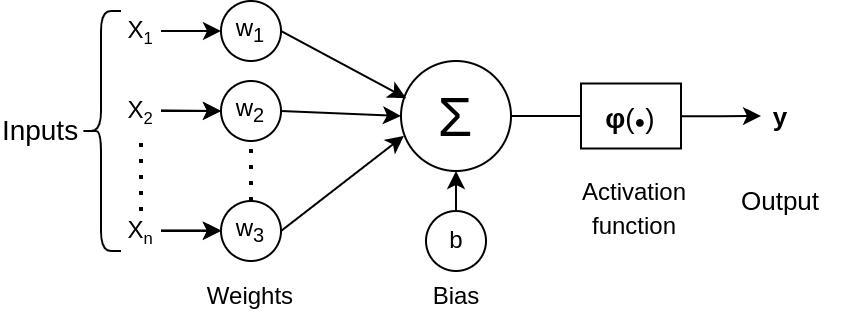
\includegraphics[width=8cm]{perceptron_diagram}
    \caption{Perceptron, the base unit of a neural network.}
    \label{fig:perceptron_diagram}
\end{figure}

Because the above result is linear, a model that only uses the above equation can only generate a linear model; thus, we use a non-linear activation function $\pmb{\varphi}$ to obtain the result of the perceptron:

\begin{align*}
    \pmb{y} = \pmb{\varphi}(C) = \pmb{\varphi}(\sum_{i=1}^n w_{i} * x_{i} + b)
\end{align*}

Although we added a non-linear function to the perceptron, a single-layer perceptron is still only capable of learning linearly separable patterns, as \citeauthor{minsky1969perceptrons} demonstrated in \citefield{minsky1969perceptrons}{title}\cite{minsky1969perceptrons} that it cannot learn an XOR function.

\begin{figure}[htp]
    \centering
    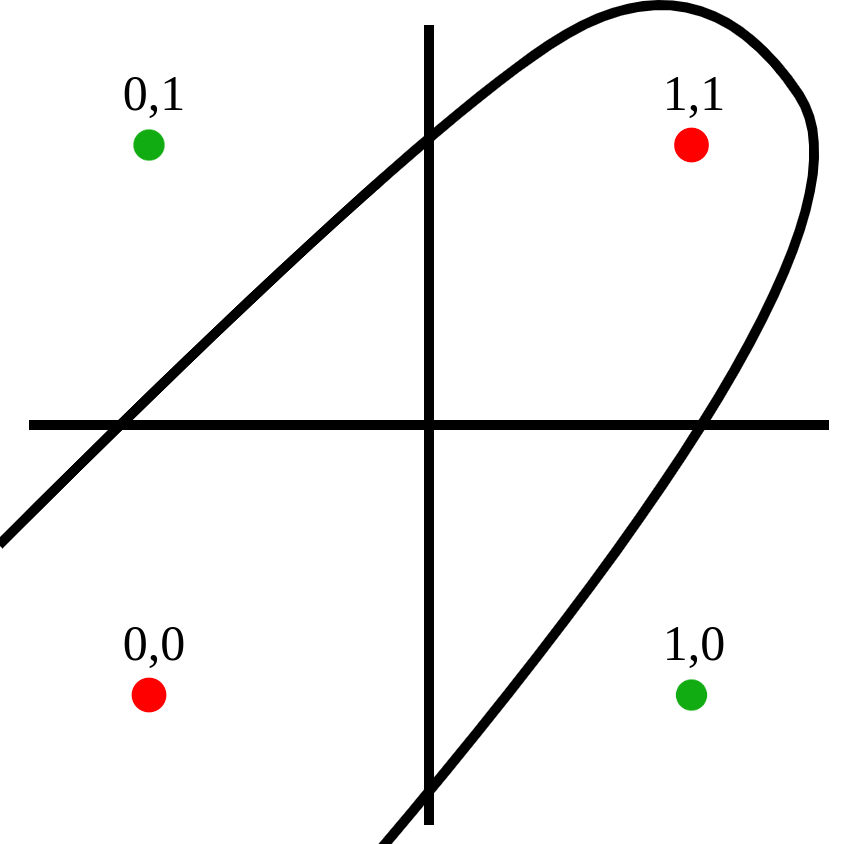
\includegraphics[width=6cm]{xor_diagram}
    \caption{A non-linear function separating the XOR pattern.}
    \label{fig:xor_diagram}
\end{figure}


There are several activation function variants, however the following are the most commonly used:

\begin{itemize}
    \item the logistic (Sigmoid) activation function, which maps input to $\left[0,1\right]$:
        \begin{align*}
            Sigmoid(x) = \sigma (x) =  \frac{\mathrm{1} }{\mathrm{1} + \mathrm{e^{-x}} } 
        \end{align*}
    \item the hyperbolic tangent (Tanh) activation function, which maps the input to $\left[-1,1\right]$
        \begin{align*}
            Tanh(x) = \frac{\mathrm{e^x} - \mathrm{e^{-x}}}{\mathrm{e^x} + \mathrm{e^{-x}}} 
        \end{align*}
    \item the rectified linear (ReLU) activation function, which maps input to $\left[0,\infty\right)$, the simplest and most commonly used function:
        \begin{align*}
            ReLU(x) = (x)^\mathrm{+} = \max(\mathrm{0}, x)
        \end{align*}
\end{itemize}

\subsection{Multi-layered perceptron}

In a neural network, the perceptron is also known as the unit or neuron. A single neuron can only solve simple tasks, but neural networks combine the power of multiple neurons arranged in layers and connected in a network architecture to solve more complex problems. This is known as a multi-layer perceptron

\begin{figure}[htp]
    \centering
    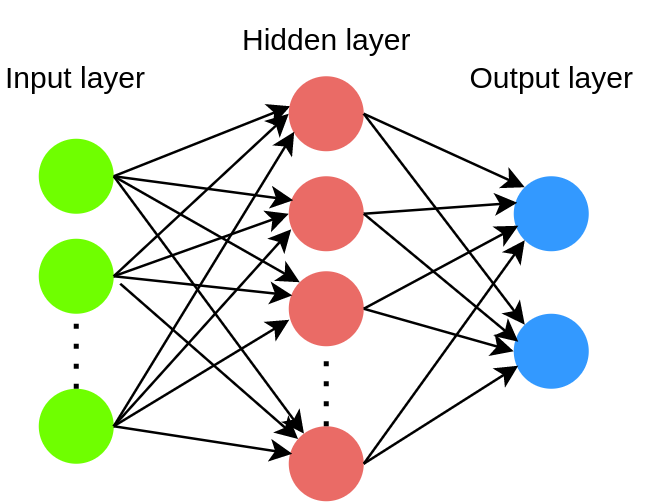
\includegraphics[width=8cm]{mlp_diagram}
    \caption{Representation of a simple multi-layer perceptron.}
    \label{fig:mlp_diagram}
\end{figure}

\textbf{The multi-layer perceptron}, like the single-layer perceptron, has an input layer with a corresponding weight on each edge leaving the input layer (see figure \ref{fig:mlp_diagram}).

There are at least three layers of nodes in an MLP: an input layer, a hidden layer, and an output layer. Each node, with the exception of the input nodes, is a neuron (perceptron) with a nonlinear activation function. The hidden layer can be extended to multiple layers so it can describe more complex linear and non-linear separable patterns of data.

\section{Convolutional neural networks}

\textbf{Convolutional neural networks} (CNN) are a class of neural networks that are most commonly used in computer vision tasks. They were first introduced by \citeauthor{lenet_paper} in \citefield{lenet_paper}{title}\cite{lenet_paper}.

CNNs, like MLPs, have at least three layers: an input layer, hidden layers, and an output layer. Despite the fact that they have the same model structure, they operate in very different ways.

\begin{figure}[htp]
    \centering
    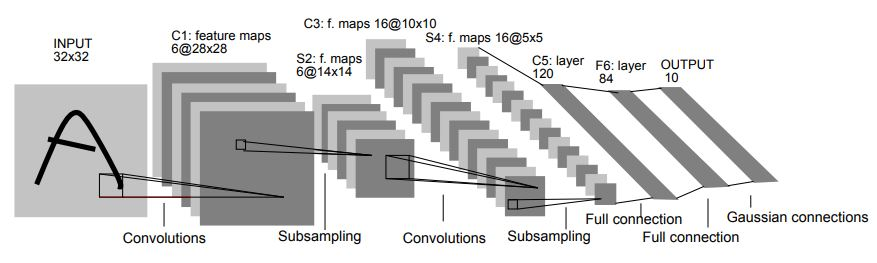
\includegraphics[width=14cm]{lenet_diagram_paper}
    \caption{Arhitecture of LeNet for digit recognition. Figure from \cite{lenet_paper}.}
    \label{fig:lenet_diagram_paper}
\end{figure}

As can be seen in figure \ref{fig:lenet_diagram_paper}, the input to a convolutional neural network is a three-dimensional tensor (first two dimensions represent the matrix and the third represents the number of channels or depth of the input, in the case of images it represents whether it's colored or grayscale).

\subsection{Layers}

A convolutional network's hidden layers typically use three types of layers: a convolutional layer, a pooling layer and a linear layer. The first two mentioned have a kernel that serves as the layer's base. The operation is performed on a patch of input that is the same size as the kernel. The squares in the figure \ref{fig:lenet_diagram_paper} represent this patch.

\subsubsection{Convolution layer}

\textbf{The convolution layer} is the main part of the CNN that transmits most of the network's information.

It is based on the mathematical operation of convolution, which is performed between a three-dimensional matrix kernel with depth and a sliding window of the layer's input (which is the output of the previous layer). The matrix size of the sliding window is determined by the kernel size and the kernel's depth is determined by the input's depth.

\begin{figure}[htp]
    \centering
    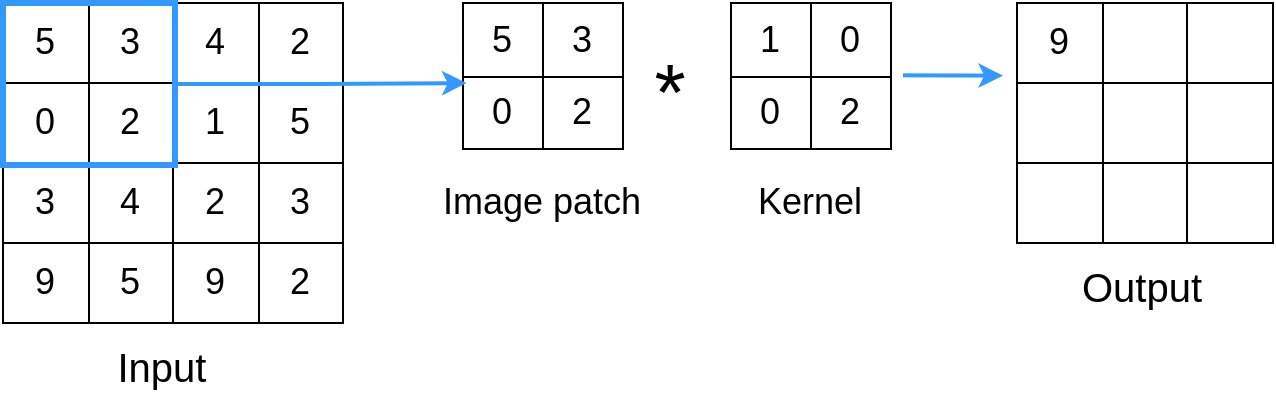
\includegraphics[width=10cm]{convolution_layer_operation}
    \caption{Represents the first step of a convolution layer operation.}
    \label{fig:convolution_layer_operation}
\end{figure}

The convolution layer just does a element-wise product between the kernel and every window of the input image, resulting in a feature map of the input in which specific information about the image is acquired like edges or corners. This operation has different parameters like padding and stride which modify the output of the new layer.

There can be multiple such convolution layers stacked on each other which produces the depth of the output.

\subsubsection{Pooling layer}

\textbf{The pooling layer} is another important component used in CNNs; its primary function is to reduce the size of the previous layer's convolved feature map. It also uses a sliding window and a kernel function that maps the output of the current window to a single value, reducing the amount of computation required in subsequent layers. This procedure is applied to each slice of the input, maintaining the depth while reducing the two-dimensional size (matrix size).

The following kernel functions are commonly used in the pooling layer:

\begin{itemize}
    \item \textbf{Max pooling}: It selects the largest number from the window.
    \item \textbf{Average pooling}: It returns the average of all the elements in the window.
    \item \textbf{Sum pooling}: It returns the sum of all the elements in the window.
\end{itemize}

\subsubsection{Fully connected layer}

\textbf{The fully connected layer} is made up of neurons with weights and biases that are fully connected with neurons from the previous and next layers. This layer is similar to, if not identical to, the multi-layer perceptron (MLP) hidden layer.

Because fully connected layers take a vector as input, the output of the final convolution layer must be linearized, so a transition layer is added in between. These layers are usually positioned immediately before the output layer.

\subsubsection{Output layer}

\textbf{The output layer} is also a fully connected layer. Because the number of neurons in this layer is equal to the number of values provided by the model, this layer is typically configured to predict the exact number of values required for our given task, whether we need to classify the input or predict specific values based on the input.

\subsection{Architectural evolution of CNN}

Despite the fact that Lecun introduced the first CNN architecture in 1998 \cite{lenet_paper}, it was not until 2012 that these types of models gained popularity. Since then, many new architectures have been introduced, but only a few have stood out.

\subsubsection{AlexNet architecture}

The convolutional neural network architecture known as AlexNet was first introduced in the paper \citefield{alexnet_paper}{title} \cite{alexnet_paper} by \citeauthor{alexnet_paper} in 2012. This was the first CNN architecture to win the ImageNet\cite{imagenet_paper} challenge, and every ImageNet challenge since then has been won by a CNN architecture that outperformed the other traditional machine learning approaches significantly.

\begin{figure}[htp]
    \centering
    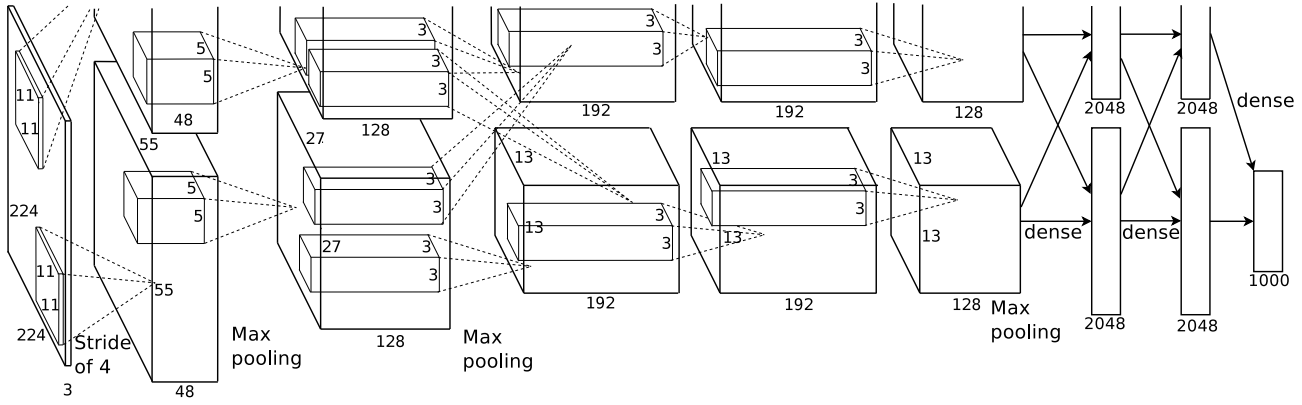
\includegraphics[width=13cm]{alexnet_diagram}
    \caption{Arhitecture of AlexNet on two GPUs. Figure from \cite{alexnet_paper}.}
    \label{fig:alexnet_diagram}
\end{figure}

The architecture is made up of eight layers, five of which are convolutional and three of which are fully connected. Despite the fact that AlexNet is very similar to the LeNet architecture, it won the ImageNet challenge without introducing any new notable technology since 1998.

AlexNet drew a lot of attention to the domain of convolutional neural networks, which are still the most popular neural networks today. They also maintain state-of-the-art status in most computer vision tasks.

\subsubsection{VGGNet architecture}

VGGNet was first introduced in the paper \citefield{vggnet_paper}{title} \cite{vggnet_paper} by \citeauthor{vggnet_paper} in 2014, and was the runner-up in the ImageNet challenge that same year.

\begin{figure}[htp]
    \centering
    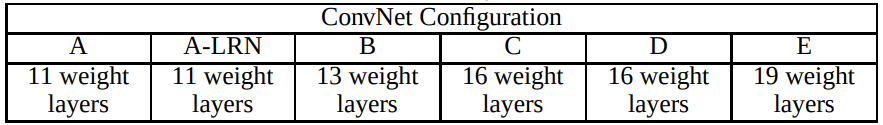
\includegraphics[width=12cm]{vggnet_layer_configs}
    \caption{Variants of the VGGNet architectures. Figure from \cite{vggnet_paper}.}
    \label{fig:vggnet_layer_configs}
\end{figure}

The main improvement it made to neural networks knowledge is that the deeper the model is, the better it can solve problems and obtain a lower error value. As a result, the VGGNet had a variety of very deep architectures, which are depicted in figure \ref{fig:vggnet_layer_configs}

However, it was later discovered that a 50+ layer depth architecture performed worse than a 20 layer architecture due to the vanishing gradient problem, so the depth of a model must be limited.

\subsubsection{GoogLeNet}

GoogLeNet was first introduced in the paper \citefield{googlenet_paper}{title} \cite{googlenet_paper} by \citeauthor{googlenet_paper} in 2014, winning the ImageNet challenge of classification that same year.

\begin{figure}[htp]
    \centering
    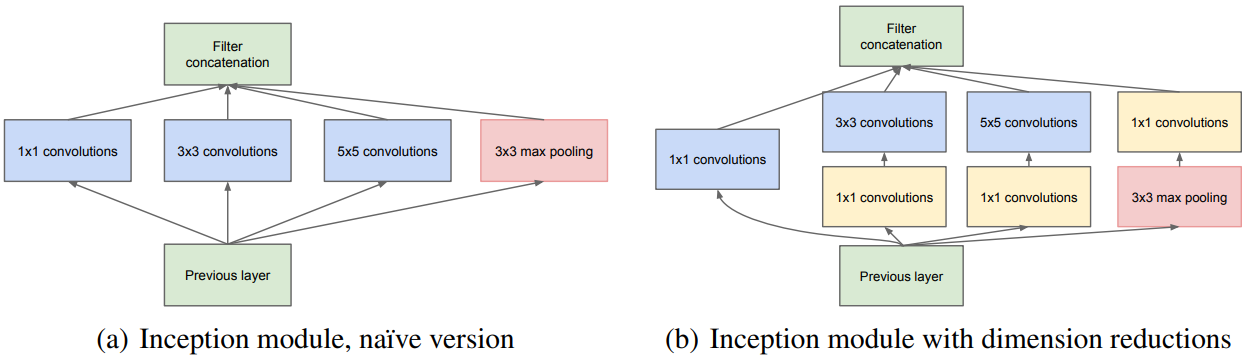
\includegraphics[width=14cm]{inception_module}
    \caption{Architecture of a inception module. Figure from \cite{googlenet_paper}.}
    \label{fig:inception_module}
\end{figure}

The authors had the same idea of using deeper models since it can produce better results, but their approach was different. They removed all fully connected layers and introduced a new structure called inception module to the the convolutional neural networks. Given that the fully connected layers were the most computationally intensive and contributed significantly more to the model's number of parameters than other layers of the CNN, this architecture is approximately 12 times smaller than Alexnet and 28 times smaller than VGGNet.

The inception module shown in figure \ref{fig:inception_module}, is based on applying different combinations of convolution and pooling layers at the same time and concatenating these outputs, which are then passed to the next layer. This method widens the model, but because the convolution and pooling operations use fewer parameters, it makes the model smaller overall.

\subsubsection{ResNet}

ResNet was first introduced in the paper \citefield{resnet_paper}{title} \cite{resnet_paper} by \citeauthor{resnet_paper} in 2015, winning the ImageNet challenge that same year.

Because of the vanishing gradient problem, models could previously have up to 20 layers without losing performance. This problem was solved by using a residual building block; as a result, models can be much deeper and perform better when using these blocks. The largest model introduced in the ResNet paper, for example, had up to 152 layers.

\begin{figure}[htp]
    \centering
    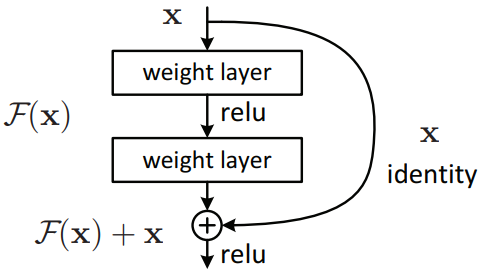
\includegraphics[width=7cm]{residual_block}
    \caption{Architecture of a residual block. Figure from \cite{resnet_paper}.}
    \label{fig:residual_block}
\end{figure}

As shown in figure \ref{fig:residual_block}, the residual block simply implements a skip connection that adds the identity of the input. With x as the input, we apply a set of layers (noted as $\mathcal{F}$) to it, yielding $\mathcal{F}(x)$ upon which we add the input (the skip connection), therefore the output is $\mathcal{F}(x) + x$.

This model popularized the concept of skip connections and is now used in many models because it solved one of the most significant drawbacks, the vanishing gradient problem.

\section{Recurrent neural networks}

Recurrent neural networks are a type of neural network that is designed to work with time series and sequential data. These networks use recurrence to process a variable length of data inputs in a sequential order, as the name implies.

\begin{figure}[htp]
    \centering
    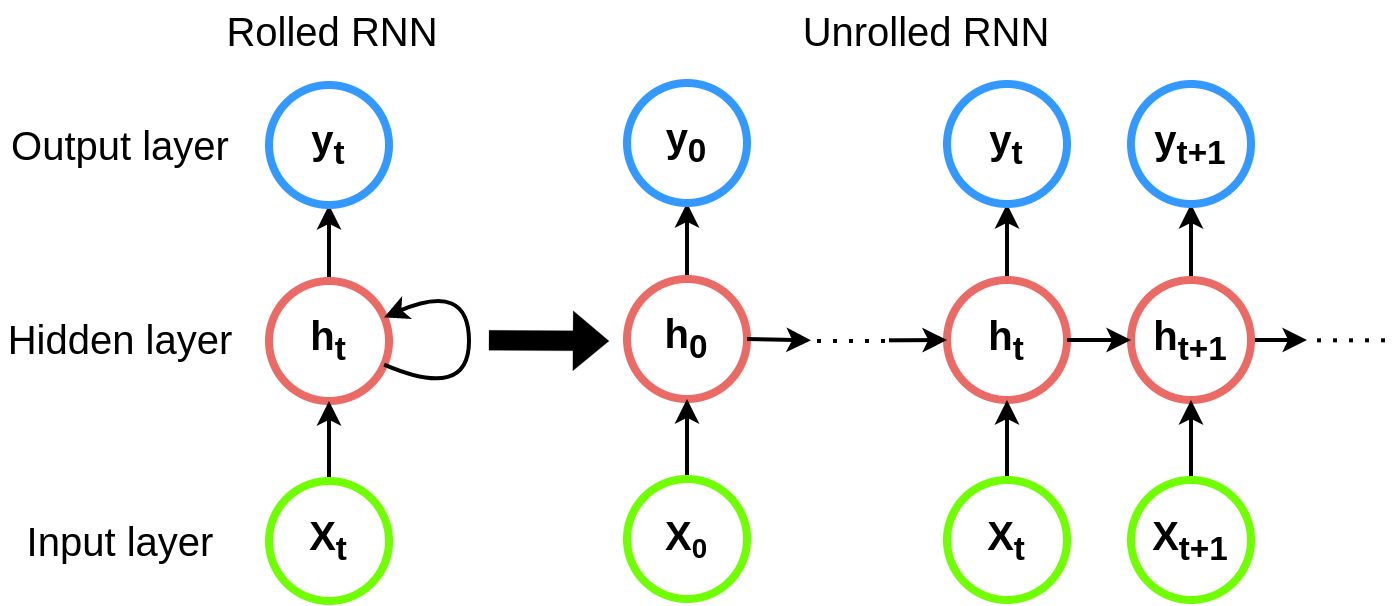
\includegraphics[width=11cm]{rnn_diagram}
    \caption{The RNN architecture, folded and unfolded representation.}
    \label{fig:rnn_diagram}
\end{figure}

As shown in figure \ref{fig:rnn_diagram}, these networks can be thought of as a recurrent extension of feed-forward neural networks, in which the neuron communicates with other neurons in the same layer.

The majority of RNN research was conducted in the field of Natural Language Processing (NLP), which is an important field that studies how computers can understand human language. Because human language is highly context-dependent, this model was ideal for the task at hand.

Recurrent neural networks use the concept of memory to store the states and information of previous inputs, which are then used to generate the new output of the sequence. Because they take the input sequentially, stacking multiple layers quickly leads to the vanishing gradient problem. To address this issue, several unit architectures have emerged, the most popular of which are: long short-term memory (LSTM) and gated recurrent unit (GRU), which perform various operations on the hidden unit $h_{t}$ memory.

\section{Training a model}

Training a neural network model refers to the process by which a neural network learns how to predict answers to problems.

\subsection{Learning methods}

Neural network models must learn how to solve tasks, and there are two main methods for doing so: \textbf{supervised learning} and \textbf{unsupervised learning}. The main difference between the two is that supervised learning employs labels in its training, which means that in addition to the input, the model also knows what the answer to that particular input is, whereas unsupervised learning uses only the input to train itself.
% There is an important difference between the two and that is supervised learning uses labels for its training, which means that besides the input, the model knows what the answer to that specific input is as well.

\textbf{Unsupervised learning} is commonly used in categories of problems like:
\begin{itemize}
    \item \textbf{Clustering}: the algorithm tries to find patterns in collections of uncategorized data, therefore it tries to make clusters (groups) of similar objects in the dataset.
    \item \textbf{Association rules}: the algorithm tries to find relationships between entries of a large dataset.
\end{itemize}

Cluster algorithms and K-means are two examples of algorithms that use this type of learning.

\textbf{Supervised learning} method is used for two big categories of problem tasks:
\begin{itemize}
    \item \textbf{Classification}: the model has to predict the correct class of the input.
    \item \textbf{Regression}: the model has to predict a value (usually continuous) that describes the solution of the problem.
\end{itemize}

\begin{figure}[htp]
    \centering
    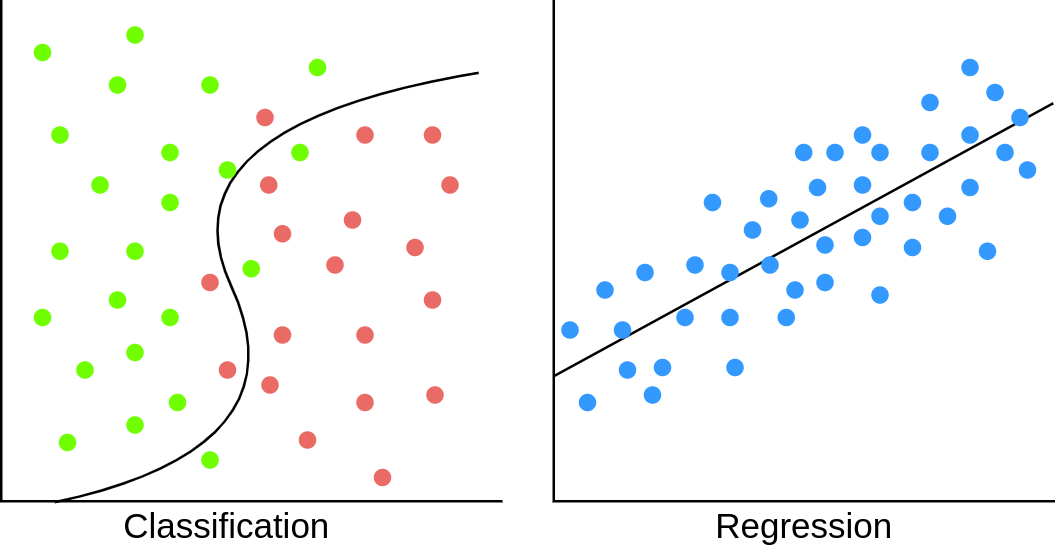
\includegraphics[width=9cm]{regression_classification_diagram}
    \caption{Classification and regression representation.}
    \label{fig:regression_classification_diagram}
\end{figure}

%like classification and regression.  If the task is a classification problem, the model must predict which class that specific input belongs to, whereas if the problem is a regression problem, the model must predict a value (usually continuous) that describes the problem solution result.

Neural networks are the most popular supervised learning models, but there are a few others worth mentioning as well: support vector machines (SVM), random forests, and linear and logistic regression.

\subsection{Training data}

Neural networks that use supervised learning to train the model require a large amount of labeled data, and it's important to note that the deeper the model gets, the more training data it requires.

In computer vision tasks, the amount of labeled data might not be enough for the model to learn enough about the task at hand; in this case, the model may be underfitting. To address this issue, we can use image augmentation, which involves making various small changes to the dataset images in order to artificially increase the size of the dataset. Although image augmentation benefits us most of the time, too much of it can lead to overfitting the model, which means it learns the training dataset far too well and is unable to predict new data properly.

Image augmentation on an input image entails performing various operations on it, such as cropping, rotating, flipping, blurring, changing the contrast, and many others.

\subsection{Backpropagation}

The algorithm was developed in the 1970s but it was popularized by \citeauthor{backpropagation_paper} in their famous \citefield{backpropagation_paper}{year} paper \citefield{backpropagation_paper}{title}\cite{backpropagation_paper}.

In neural networks weights determine how the output of the network will be. 

In a \textbf{forward pass}, the neural network runs the input through all the layers, and the weighted layers perform the operation that was designed for them, which is usually a product between the weights of the layer and the input of the layer (which is the output of the previous layer), to which a bias can be added. The last layer, the output layer produces the results of the neural network.

We have the outputs of the entire neural network after the forward pass, and a \textbf{loss function} connects the forward and backward passes. A loss function's main task is to calculate the error or loss of the neural network's output in relation to the real values, or labels, of the input data.

The loss function varies greatly depending on the task, but here are a few examples:

\begin{itemize}
    \item \textbf{Mean absolute error loss}: measures the L1 norm between the output and the label.
    \item \textbf{Mean square error loss}: measures the L2 norm between the output and the label.
    \item \textbf{Cross entropy loss}: it is used in classification, particularly when there are several classes. It computes the loss of the model class probability predictions (typically predicted with softmax) given the input's actual class.
\end{itemize}

Once we have the outputs and calculated the loss with the loss function, only on training the backward pass is up next. 

The \textbf{backward pass} employs a backpropagation algorithm, which is typically based on the chain rule. The chain rule is a part of calculus theory, and it can be expressed in Leibniz's notation as follows: if a variable z depends on y, which depends on a variable x, then z depends on that x variable through the intermediate y, which can be expressed as:
\begin{align*}
    \frac {dz}{dx} = \frac {dz}{dy} \, \frac {dy}{dx}
\end{align*}
Backpropagation propagates loss function gradients back to all weights in the model by calculating the derivative of the loss function in relation to a specific weight layer, which can be obtained using the chain rule. Backpropagating the model's gradients causes the network's weights and biases to adjust in such a way that the loss function is minimized.

Algorithms that decide how the gradients are propagated backwards are usually called \textbf{optimizers}. Because gradients can become large during the backpropagation pass, all optimizers have a \textbf{learning rate} that determines how much of the gradient will contribute to the weights.

 \textbf{Gradient Descent} was one of the first and most popular optimizer. It employs first order derivatives, which can be thought of as the gradient, and simply subtracts them from the weights based on a learning rate $\alpha$:
\begin{align*}
    \theta = \theta - \alpha * \nabla f(\theta)
\end{align*}

Aside from gradient descent, there are several algorithms that propagate the gradient in various ways, the most notable of which are:
\begin{itemize}
    \item \textbf{Stochastic gradient descent (SGD)}: similar to gradient descent, but the weights are updated more frequently, once per training batch or input.
    \item \textbf{Adaptive gradient (AdaGrad)}: this optimizer updates both the learning rate and the weights. One issue with this optimizer is that if there are too many iterations, the learning rate becomes too small and the model stops learning.
    \item \textbf{AdaDelta}: it updates the learning rate similarly to AdaGrad, but it uses a better method that solves the AdaGrad problem by updating the learning rate with a moving window of gradient updates.
    \item \textbf{RMSprop}: similar to AdaDelta, it also uses an exponentially decaying average of squared gradients.
    \item \textbf{Adaptive movement estimation (Adam)}: one of the most powerful optimizers, can be thought of as a hybrid of RMSprop and SGD with momentum.
\end{itemize}

\section{Transformer}

The transformer was first presented in the paper \citefield{attention_is_all_you_need}{title}\cite{attention_is_all_you_need} by \citeauthor{attention_is_all_you_need} from Google in \citefield{attention_is_all_you_need}{year}, in which they presented the transformer's base structure, which is an encoder-decoder architecture based on a new layer called attention layers.

% It was initially introduced for tasks specifically in the domain of the natural language processing (NLP) and the paper targeted a machine translation task. The transformer goal was to improve the way RNN networks worked, especially in the perspective of the sequential input. That's why this model has attention that is similar to the RNN's memory but its input is parallel, all the data can be fed at once in the model.

It was first introduced for tasks in the natural language processing (NLP) domain, and the paper focused on a machine translation task. The transformer's goal was to improve the performance of RNN networks, particularly in terms of sequential input. As a result, this model has attention similar to RNN memory, but its input is parallel, allowing all data to be fed into the model at the same time. 

This model can learn to pay attention to specific parts of the whole sequence from the perspective of a token. For example in the statement: "The dog is very small but it can run fast." because both tokens refer to the same entity, the token for the word "it" would pay the most attention to the token of "dog".

\begin{figure}[htp]
    \centering
    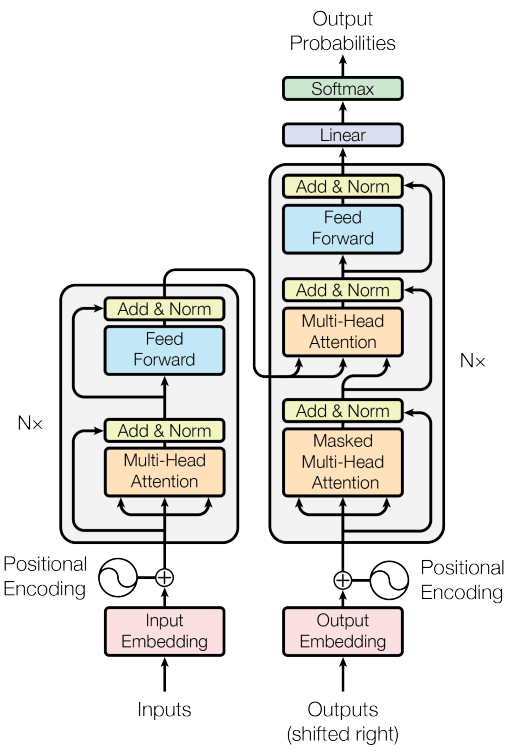
\includegraphics[width=9cm]{transformer}
    \caption{The transformer architecture. Figure from \cite{attention_is_all_you_need}.}
    \label{fig:transformer}
\end{figure}

As we can see in figure \ref{fig:transformer}, the transformer has two main parts, the encoder and the decoder.

Tokens (which usually represent words) are fed into the transformer and then passed through a layer called input embedding, where a positional encoding is applied before being sent to the encoder.

The input embedding layer maps the token sequence $x=(x_{1}, x_{2}, \dots, x_{n})$ to a continuous representation called embedding $z=(z_{1}, z_{2}, \dots, z_{n})$. The $d_{model}$ embedding size is maintained throughout the encoder and decoder layers.

In most cases, the positional encoding that is added to the input embeddings is learned, but \citeauthor{attention_is_all_you_need} tried a fixed one based on sinusoidal functions, which was later shown to be inferior to the learned one:
\begin{align*}
    PE_{(pos, 2i)} = \sin{\frac{pos}{10000^{\frac{2i}{d_{model}}}}}\\
    PE_{(pos, 2i+1)} = \cos{\frac{pos}{10000^{\frac{2i}{d_{model}}}}}
\end{align*}
Positional encoding is critical because this model is supposed to have attention, which means it must remember the input and context around a specific token. Because the model's input is all fed at once, it lacks a sense of order and position; thus, positional encoding was a necessary induced bias to the model.

Obtaining the embeddings and adding the positional encoding is thus required before feeding it to the model's first component, the encoder.

\begin{figure}[htp]
    \centering
    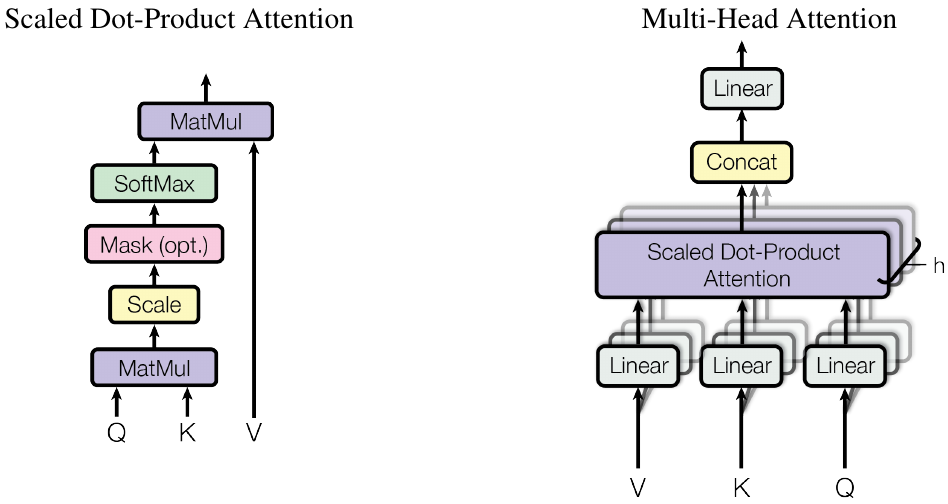
\includegraphics[width=13cm]{transformer_mha}
    \caption{ The Scaled Dot-Product Attention (left) and the Multi-Head Attention (right). Figure from \cite{attention_is_all_you_need}.}
    \label{fig:transformer_mha}
\end{figure}

\textbf{The encoder} takes as input a sequence of vectors of size $d_{model}$ and outputs a set of vectors of same size with accumulated information and attention about itself and the rest of the sequence. The encoder is made up of two main sublayers, as shown in the left part of figure \ref{fig:transformer}. The first is a multi-head self-attention mechanism and the second is a simple fully connected feed-forward network.

% \textbf{The Multi-Head Attention} is the most important component of this model. This structure takes three vectors as input: the query (Q), keys (K) and values (V). These vectors are usually linearly projected from the encoder's input vector (of a single token). Despite the fact that they can be projected to different sizes, most models use the same $d_{model}$ as the embeddings.
\textbf{The Multi-Head Attention} is the most important component of this model. This structure takes three vectors (for simplicity we will consider them vectors) as input: the query (Q), keys (K) and values (V). These vectors are usually linearly projected from the encoder's input vector (of a single token). Despite the fact that the query and keys can be projected to a $d_k$ dimension and the values to a $d_v$ dimension, which can differ from the $d_{model}$ dimension, most of the models simply consider $d_k = d_v = d_{model}$ and that's what we will assume as well.

% As we can observe in the right side of figure , these three vectors can be further linearly projected in $h$ heads of size ${d_{model}}/{h}$ before being further passed to the scaled dot-product attention. In practice the Q, K and V are actually matrices where each line corresponds to a a single token from the input sequence. Therefore it is more efficient from a complexity perspective to split these matrices in smaller parts, since it reduces the computation cost, similar to the idea presented in \cite{factorization_tricks_for_lstm_networks}.

These three vectors can be further linearly projected or just split in $h$ heads of size ${d_{model}}/{h}$ before being passed to the scaled dot-product attention, as shown on the right side of figure \ref{fig:transformer_mha}. The Q, K, and V are actually matrices, with each line representing a single token from the input sequence. As a result, splitting these matrices into smaller parts is more efficient from a complexity standpoint, as it reduces the computation cost, similar to the idea presented in \cite{factorization_tricks_for_lstm_networks}.

After the matrices are split and passed through the scaled dot-product attention, the outputs are concatenated and then, optionally linearly projected to the $d_{\text{model}}$ dimension. 

These linear projections before and after the dot-product attention are intended more for the case where the $d_k \neq d_{\text{model}}$, respectively $d_v \neq d_{\text{model}}$, but even in the case of $d_k = d_v = d_{model}$ these linear layers provide learning weights, therefore the model can learn more.

This structure operations can be represented as:
\begin{align*}
    {\text{MultiHead}}(Q, K, V) = \text{Concat}\left(\text{head}_1, \dots, \text{head}_h\right)W^O\\
    \text{where}\ \text{head}_i = \text{DotProduct}\left(QW_i^Q,KW_i^K,VW_i^V\right)
\end{align*}
where $W_i^Q, W_i^K, W_i^V \in R^{d_{\text{model}}\times d_{\text{model}}/h}$ and $W^O\in R^{d_{\text{model}}\times d_{\text{model}}}$.

\textbf{The Scaled Dot-Product Attention} is the base operation in the multi-head attention. This structure takes as input three matrices Q, K, V as shown on the left side of figure \ref{fig:transformer_mha}. 

This structure has no learning layers; its primary function is to perform the transformer's attention, which is accomplished by performing a series of operations on the inputs. It starts by doing a dot product between the query and transpose keys matrices. This operation produces a new matrix of dimension $N\times N$ (N being the number of tokens in the sequence). The initial matrices were standardized, but because the new matrix's standard deviation is $\sqrt{d_{model}}$, it no longer holds that property. After dividing the matrix by the scalar $\sqrt{d_{model}}$, each line of the matrix is subjected to a softmax. Finally, we multiply this matrix by the V matrix to get the scaled dot-product attention output.

The operation of this layer can be represented as:
\begin{align*}
    {\text{Attention}}(Q, K, V) = \text{softmax}\left(\frac{QK^{T}}{\sqrt{d_{\text{model}}}}\right)V
\end{align*}

As a result, the encoder's input is passed through the first sublayer, multi-head attention, to whose output we add a residual connection and normalize it to allow for deeper models. Then we pass it through the second sublayer, a simple feed forward network (which consists of two linear transformations with a ReLU activation function in between them), upon which we add the residual connection and normalize again. These encoder layers can be stacked multiple times, for example medium-sized networks have 12 encoder layers stacked.

\textbf{The decoder} can also have stacked identical layers. It has one more sublayer than the encoder, which receives the output of the last encoder layer, as shown in figure \ref{fig:transformer}.
This layer uses masked multi-head attention, which masks the output embeddings so that a token from the output can only access past tokens relative to time sequence.

The transformer is a very powerful model that can generalize data very well and understand context very well, and it can also be used for more than one task. Because of its flexibility, this model can be used to solve multiple task-solving problems without losing accuracy when compared to as it was trained for a single task. Even though it is very powerful, it is also a very large model that requires a lot of resources and time to train.

One of the most significant advantages of this model is that it is trained in a self-supervised manner using various methods, and when it is required to be used on a specific task or dataset, it can be easily fine-tuned, a process that is much faster than the training itself. This approach gives very good results on small datasets as well.

Many models that have been released since the initial transformer paper have only used the encoder part of the model, particularly in the computer vision field.

\chapter{Recent work}

Despite the fact that transformers have recently become highly popular, there are still very few articles that specifically explore the template matching task.

\section{Template matching}

Because computer vision is a very popular field, there have been many solutions to the task of template matching over the years.

Recent improvements and applications in the template matching area are discussed in paper \cite{template_matching_methods_paper}, although they mostly present methods based on the naive template matching algorithm, which typically employs a sliding window to discover templates which further calculates a similarity.

There are a few studies that aim to employ deep learning to solve the problem of template matching, although the majority of them use a CNN-based architecture.

The authors of the paper \cite{robust_template_matching_paper} present a training technique based on the CaffeNet\cite{caffenet_paper} architecture that employs a single model. The model is first pre-trained on a multi-view dataset, which contains multiple images of a template from different perspectives and angles that do not overlap. During pre-training, the model employs a classifier to predict those templates. When the actual dataset is fine-tuned, the classifier is replaced with a new one that corresponds to the new classes. Essentially, they use the idea of learning the features of the templates and then using that model to fine-tune on the new task, a similar idea to ours, but with a different approach.

The model presented in \cite{deep_object_template_matching_paper} employs a number of high-quality models to carry out various tasks that lead to template matching. Given the input image, it first employs the convolutional-based model SSD\cite{ssd300} to detect and extract objects from it. Then it employs a ResNet\cite{resnet_paper} model to classify the images into classes, following which it employs a gradient-based algorithm to template match the classified object with the template that represents the class.

The QATM model \cite{qatm_paper} is based on a feature extractor and similarity functions. Given the feature maps produced by the feature extractor of the image and the template, the idea presented in this paper calculates a similarity score between the two maps and then uses the QATM measurement to generate regions of interest that represent the template matchings.

% There are many papers that treat the problem of person re-identification using tansformers like \cite{aatransformer_paper}\cite{transreid_paper}  that use various ideas, that are mostly based on the modification of the transformer encoder layer, but it presents ideas that could be applied in the template matching field as well.

The AAformer\cite{aatransformer_paper} and TransReID\cite{transreid_paper} are two publications that deal with the subject of person re-identification using tansformers. The AAformer is a tranformer-based model that altered the architecture of multi-head attention so that it selects only a subset of patches that represent a specific zone of the template, thus paying more attention to a specific part of the person. This concept can also be applied to templates, so this method approaches the domain of template matching indirectly. The TransReID has a similar idea in which it just shuffles the patches instead of choosing just a subset.

\section{Vision transformer}

Vision transformers have recently received a lot of interest, especially with the state-of-the-art results especially in image classification. The ViT model is at the heart of most recent works in the computer vision field that use transformers.

% The DINO model \cite{dino_paper} is based on the ViT transformer but applies a different learning approach which is based on knowledge distilation and self-supervised learning. Therefore this model doesn't require a dataset with labels for training and also uses a teacher-student learning approach where the teacher is based on the student.

The BEiT\cite{beit_paper} transformer model was the first to successfully employ the self-supervised learning technique, which produced better results than the supervised approach. It is based on the masked image modelling (MIM) task, which employs blockwise masking to mask image patches, which it later tries to reconstruct. This method is very similar to the BERT\cite{bert_paper} model's masked language modeling (MLM), one of the most used techniques in natural language processing field. Later, ViTMAE\cite{vitmae_paper} model took a similar approach, masking entire image patches and then attempting to reconstruct the pixel values of those masked patches.

The DINO model \cite{dino_paper} is built on the ViT transformer but takes a distinct approach to learning that is focused on knowledge distillation and self-supervised learning. This model introduced a self-distilation method that employs a teacher and a student network, but the teacher is created based on the student network.

Recent works like DETR\cite{detr_paper} and YOLOS\cite{yolos_paper} have successfully created a transformer that can predict multiple objects and their classes. Both models use a set of MLP heads to predict the bounding box and whether or not an object exists within it and then it predicts a class as well. Despite using vision transformers, these models perform worse than current state-of-the-art CNN-based models such as YOLO\cite{yolo_paper} and Faster R-CNN\cite{faster_rcnn_paper}.


\chapter{Technologies used}

The technologies utilized to implement the siamese model described in this thesis are presented in this chapter.

\section{Python}

\textbf{Python} is a well-known and widely used high-level programming language. This programming language is interpreted and object-oriented, and it has excellent support for modules and packages, resulting in a wide range of libraries.

Python is an amazing programming language because it allows us to create complex algorithms with little effort and also has a lot of flexibility since it is a dynamically typed language.

This programming language offers the most support for machine learning applications, with a large number of libraries dedicated to the field. Specifically for neural networks, there are three main frameworks used: TensorFlow, Keras and PyTorch. In my implementation I decided to use PyTorch.

\section{PyTorch}

\textbf{PyTorch}, based on the Torch library, is an open source machine learning framework primarily for Python. It was designed specifically for deep learning and can be used on both the GPU and CPU. Low-level languages are used to implement the most important computation-related code, ensuring that it is implemented as efficiently as possible.

One of the most important features it offers is tensor computation with strong GPU acceleration. A tensor is simply a multidimensional array (similar to a NumPy array) that can be stored on both the CPU and the GPU and has various operations implemented.

PyTorch makes it simple to build neural network models from scratch and works well with other Python modules such as NumPy.

\section{HuggingFace}

\textbf{HuggingFace} is one of the biggest and most popular transformer library. Most of the biggest companies like Google, Facebook, Nvidia and others post some of the best and newest trained models in this library. It's mainly built on top of the PyTorch framework but it also has support for TensorFlow.

Since transformer models are very hard to train, it is important to be able to obtain pre-trained transformers, so that it can be later fine-tuned on the specific tasks at hand. HuggingFace provides most of the state-of-the-art models which can be downloaded and imported in a project very easily.

\section{Notable libraries}

There are some other notable libraries that I have used in my project:
\begin{itemize}
    \item \textbf{NumPy}: a popular library that provides a multidimensional array object and other derived objects upon which many optimized computing operations are implemented.
    \item \textbf{Pillow (PIL)}: used for image format support and image processing.
    \item \textbf{Pandas}: used for data analysis and manipulation tool.
    \item \textbf{Matplotlib}: used for creating plots and other visualizations in python.
\end{itemize}

\chapter{Proposed approach}

\section{Concept}

Transformer models have a large number of parameters and require a large amount of hardware resources when training, which is impossible with my current computational resources, so I chose to use a pre-trained model on which I applied the process of fine-tuning down the specific task of template matching.

\begin{figure}[htp]
    \centering
    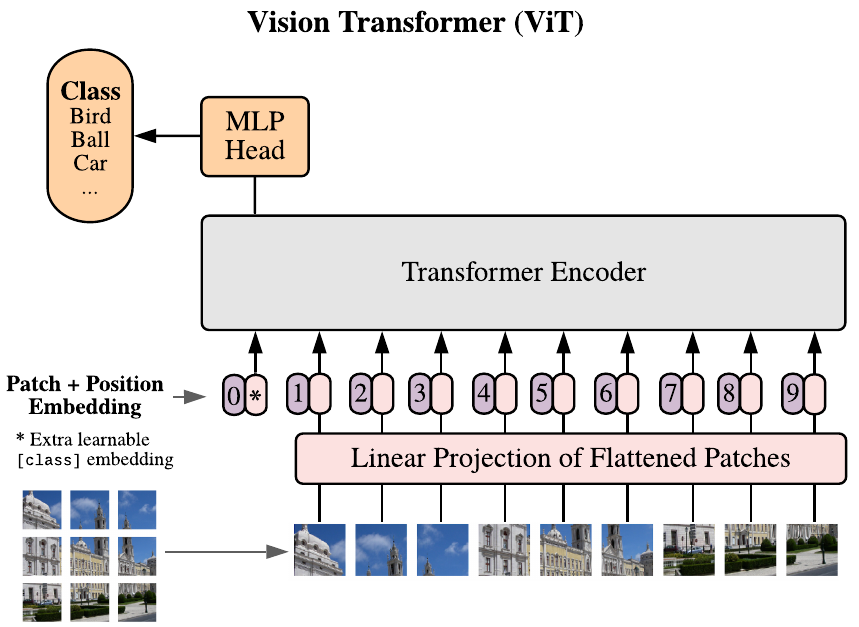
\includegraphics[width=11cm]{vit_transformer}
    \caption{The ViT Transformer on training. Figure from the ViT paper \cite{vit_paper}.}
    \label{fig:vit_transformer}
\end{figure}

To solve the proposed problem, I will use models with a specific architecture that allows for images as input type; these models have also been pre-trained on large datasets of images.


The task of template matching has two images as input data, but as shown in figure \ref{fig:vit_transformer}, a model of type vision transformer can only receive one image as input; also, given that the model is pre-trained in this manner, we can assume it would not perform well if we tried to use only one model and concatenate the inspected image and the template image together and use it as input (as BERT\cite{bert_paper} does).

As a result, I concluded that the best way to solve this task with transformers is to use a Siamese architecture.

\section{Vision Transformer}

The Vision Transformer (ViT) \cite{vit_paper} is the main transformer model that I have used in my experiments.

\begin{figure}[htp]
    \centering
    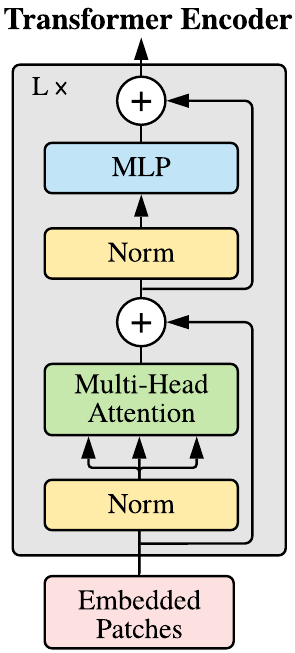
\includegraphics[width=4cm]{vit_encoder}
    \caption{The Transformer Encoder used in ViT. Figure from the ViT paper \cite{vit_paper}.}
    \label{fig:vit_encoder}
\end{figure}

As shown in figure \ref{fig:vit_transformer}, this model takes an image or a batch of images as input and splits each image into fixed-size patches that do not overlap, without losing any part of the original image. 

% After it has the patches they are fed into the "Linear Projection of Flattened Patches" layer. This layer is described by the authors of the paper as simply unrolling the matrix of each patch in a very long linear array which is then mapped using a trainable linear projection to patch embeddings. In more mathematical terms this means that the patch array is multiplied by a big matrix that maps the patches from the initial dimension to the embedded dimension.

The patches are then fed into the "Linear Projection of Flattened Patches" layer. The authors of the paper describe this layer as simply unrolling the matrix of each patch in a very long linear array, which is then mapped to patch embeddings using a trainable linear projection. More precisely, the patch array is multiplied by a large matrix that maps the patches from the initial dimension to the embedded dimension $d_{\text{model}}$.

As shown in figure \ref{fig:vit_transformer}, the ViT model, like many other transformers, has a 0-indexed embedding that represents the class learnable embedding known as the [CLS] token. This is a critical model embedding because its primary goal is to gain a global understanding of all the patches and thus of the entire image.

Therefore the input of the ViT encoder are all the patch embeddings concatenated with the [CLS] embedding token.

The encoder layer in the ViT model is the same as the one presented by Vaswani et al. in the original transformer paper \cite{attention_is_all_you_need}. Given the embeddings it runs them through multiple stacked encoder layers. Each encoder layers has two sub-layers, the Multi-Head Attention (MHA) layer and a multilayered perceptron (MLP) layer as shown in figure \ref{fig:vit_encoder}. The encoder also has normalization preceding the two sub-layers and the residual connections added to the output of these sub-layers.

The encoder layers are the most important part of the model because they apply global attention to all of the image's patches, and the final layer's output will be a vector containing features of different objects in the image and their relationships for each patch that was given as input.

But as we can see in figure \ref{fig:vit_transformer} the model was trained using only the [CLS] token output which has the global understanding of the image, therefore I only use the feature vector produced by the [CLS] token, which represents a global understanding of the image.

\section{Fine-tuning a model}

In the transformers models, fine-tuning is a very common process.

% As shown in figure \ref{fig:fine_tuning} the main idea of fine-tuning is given an already trained model we add a new task that's untrained yet and we remove or keep the old task solvers. When we train the new task and keep the old weights of the model, what we are actually doing is fine-tuning the weights of the whole model (it already has a base way of learning from images) and train from zero only the new task. This process works very well when the old tasks are similar with the new task, otherwise this training procedure won't have a good performance.

The main idea of fine-tuning is to take an already trained model and add a new task that hasn't been trained yet, while removing or keeping the old task solvers, as shown in figure \ref{fig:fine_tuning}. When we train the new task while keeping the old model weights, we are actually fine-tuning the weights of the entire model (it already has a base way of learning from images) and only training the new task from zero. This process works best when the old and new tasks are similar; otherwise, this training procedure will not be effective.

We use fine-tuning in our work because it has several advantages, particularly in the case of vision transformers:

\begin{itemize}
    \item it needs less data for model training because the process of fine-tuning a transformer allows it to get good results on small datasets with a very large model.
    \item requires less train time and computation, fine-tuning a transformer can take a few hours or even minutes compared to the training time of ViT model which is equivalent to a few hundred days on a TPUv3 core \cite{vit_paper}.
\end{itemize}

\begin{figure}[htp]
    \centering
    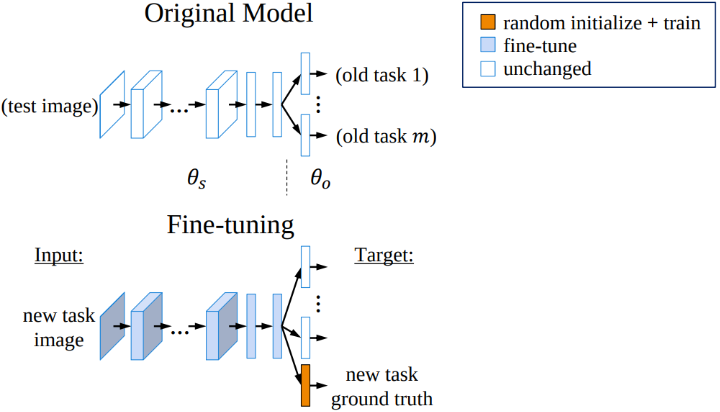
\includegraphics[width=11cm]{fine_tuning}
\caption{Representation of fine tuning. Figure from \cite{learning_without_forgetting}.}
    \label{fig:fine_tuning}
\end{figure}


\section{Siamese model}

\begin{figure}[htp]
    \centering
    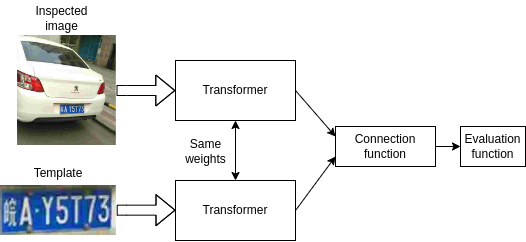
\includegraphics[width=12cm]{siamese_transformer}
    \caption{Representation of a general siamese network using transformer.}
    \label{fig:siamese_transformer}
\end{figure}

A Siamese architecture entails using multiple identical networks with the same structure and weights to generate a feature vector from multiple different inputs and then performing some operations on those outputs.

Siamese networks are mostly used for similarity problems, more exactly to compare two or more feature vectors of different inputs and optionally apply some other tasks on top of the model.

%\item \textbf{Cosine embedding loss}: given two input tensors, and a label which represents if the tensors are the same or not, it creates a criterion that uses cosine similarity to measure the similarity of dissimilarity between the two tensors.

\section{First proposed model}

Template matching has as input two images, the inspected image and the template.

Although the vision transformer is the state-of-the-art for most single-image classification tasks, current transformer-based multiple object detection approaches are inferior to CNN-based state-of-the-art models.

As a result, we will use only the [CLS] feature vector to look for a single instance of the template in the inspected image.

\begin{figure}[htp]
    \centering
    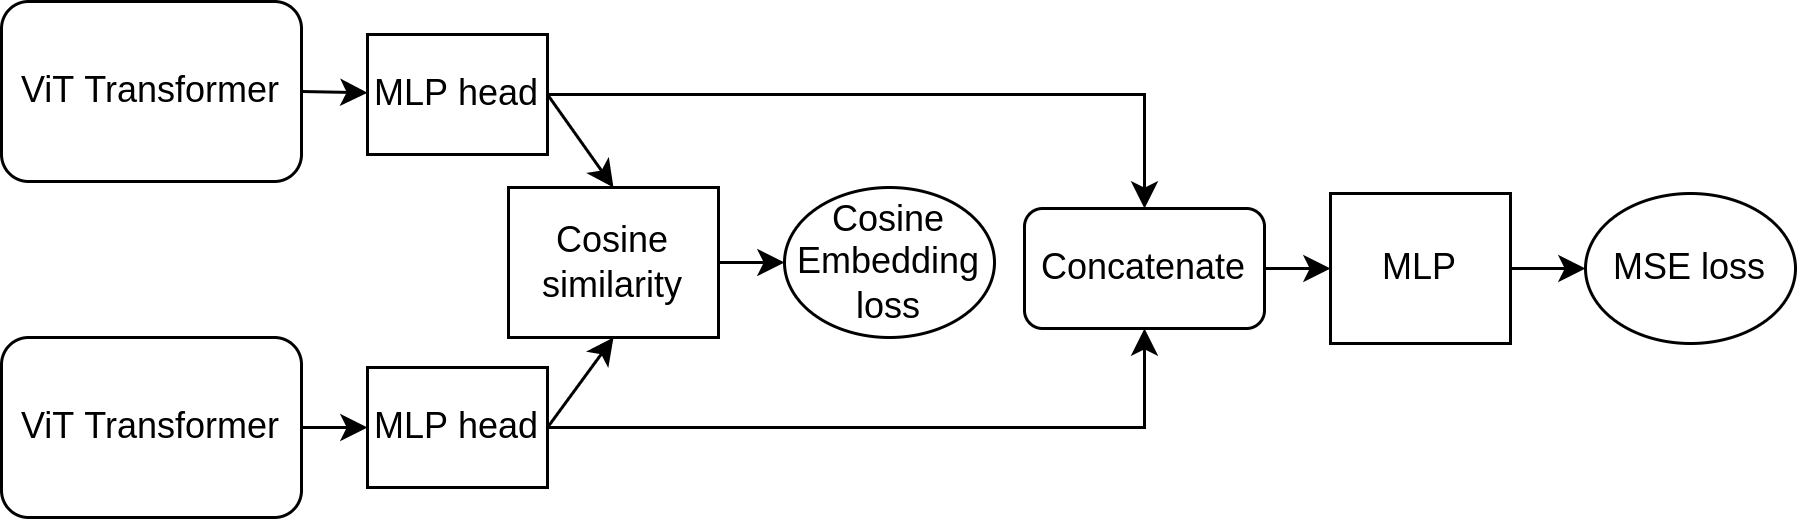
\includegraphics[width=14cm]{first_approach_diagram}
    \caption{The diagram of the first model, two siamese transformers with classification and regression heads.}
    \label{fig:first_approach_diagram}
\end{figure}

Our model uses the two ViT transformer encoders to process the image and template, as shown in figure \ref{fig:first_approach_diagram}. The output of the transformer is a sequence of feature vectors of length  $d_{\text{model}}$, corresponding to the [CLS] token and all patch embeddings. For both the image and the template, as previously mentioned, only the feature vector of the [CLS] token will be extracted from this matrix and passed onward.

I decided to add an MLP head on top of the transformers, as the original ViT paper had, but that would keep the same dimension $d_{\text{model}}$ of the feature vector. Though this addition only marginally improved the model's results; thus it can be omitted.

As a result, for both the image and the template sides, only the extracted feature vector is fed into the MLP head, yielding the final features that describe them.

Now that we have the final feature vectors for both the image and the template, we want to calculate the similarity of the two images and, eventually, predict whether or not the template is present in the inspected image. To determine how similar the feature vectors are, we compute the cosine of the angle between the two vectors, which represents whether the vectors are pointing in the same direction. Given the feature vectors $x_{1}, x_{2}$, the cosine similarity formula is:
\begin{align*}
    \text{cosine\_similarity}\left(x_{1}, x_{2}\right) = \frac{x_{1}\cdot x_{2}}{\max\left(\left\lVert x_{1}\right\rVert_2\cdot \left\lVert x_{2}\right\rVert_2, \epsilon\right)}
\end{align*}
where $\epsilon$ is a small constant that guarantees we will not divide by zero.

The value obtained above is one of the model's outputs, which takes values in the interval $\left[-1,1\right]$, which can be interpreted as:
\begin{itemize}
    \item $-1$ represents an angle of $180^{\circ}$
    \item $0$ represents an angle of $90^{\circ}$
    \item $1$ represents an angle of $0^{\circ}$
\end{itemize}
As a result, a value close to 1 indicates that the images are similar, while a smaller value indicates that the images are dissimilar.

The model must figure out how to group similar images and templates together and spread out the ones that aren't. As a result, a loss function is required, and our model employs cosine embedding loss.

The cosine embedding loss is a criterion that calculates the loss based on the two feature vectors and a label $y$ that takes values of 1 or -1, indicating whether the template is present in the image or not. Its formula, which is based on the cosine similarity function, is as follows:
\begin{align*}
    \text{loss}(x, y) =
        \begin{cases}
        1 - \text{cosine\_similarity}\left(x_1, x_2\right), & \text{if } y = 1 \\
        \max(0, \text{cosine\_similarity}\left(x_1, x_2\right) - \text{margin}), & \text{if } y = -1
        \end{cases}
\end{align*}
In the case when the template is found in the image ($y=1$) the loss subtracts from 1 the cosine similarity, resulting in a loss that is close to 0 if they are similar and close to 2 if they are not. In the opposite case of $y=-1$ we subtract a margin from the cosine similarity and ensure that the resulting value is positive.

I've also attempted to use a different loss function instead of the cosine embedding loss, which is the contrastive loss function described in \cite{contrastive_loss_paper} but the model performed worse with this loss function.

The purpose of the first part of the model is to simply introduce a similarity and dissimilarity concept into the ViT transformer, allowing the model to predict whether or not the given template can be found in the inspected image.

This model also tries to predict where the template will be found in the inspected image using bounding box prediction. To do so, we first concatenate the two feature vectors produced by the two MLP Heads that correspond to the inspected image and the template, as shown in figure \ref{fig:first_approach_diagram}.

The concatenated feature vector of size $2\cdot d_{\text{model}}$ is then fed to an MLP layer, whose output is a linear layer with four neurons that represents bounding box coordinates scaled to the interval $\left[0,1\right]$. These coordinates represent the two corners of the box, top left $\left(x_1,y_1\right)$ and bottom right $\left(x_2,y_2\right)$, in which the model predicts the template will be found.

The model must also learn how to predict the bounding box, so we need a loss on these four coordinates. I chose the mean squared error (MSE) loss function, which computes the squared L2 norm between the model's output vector $x$ and the label vector $y$ of the same size:
\begin{align*}
    \sum_{i=1}^{4}(x_i-y_i)^2
\end{align*}

As a result, the model learns via backpropagation, and the loss function in our case is composed of two loss functions, the cosine embedding loss and the MSE loss. During training, we add these losses and backpropagate them.

This model holds the exact same structure on evaluation, the only difference being that we obviously don't backpropagate the gradients anymore.

One significant drawback of this model is that it attempts to predict the bounding box during training even when the template is not present in the image, resulting in unnecessary gradients that change the weights during training. I proposed the following model as a solution to this problem.

\section{Second proposed model}

\begin{figure}[htp]
    \centering
    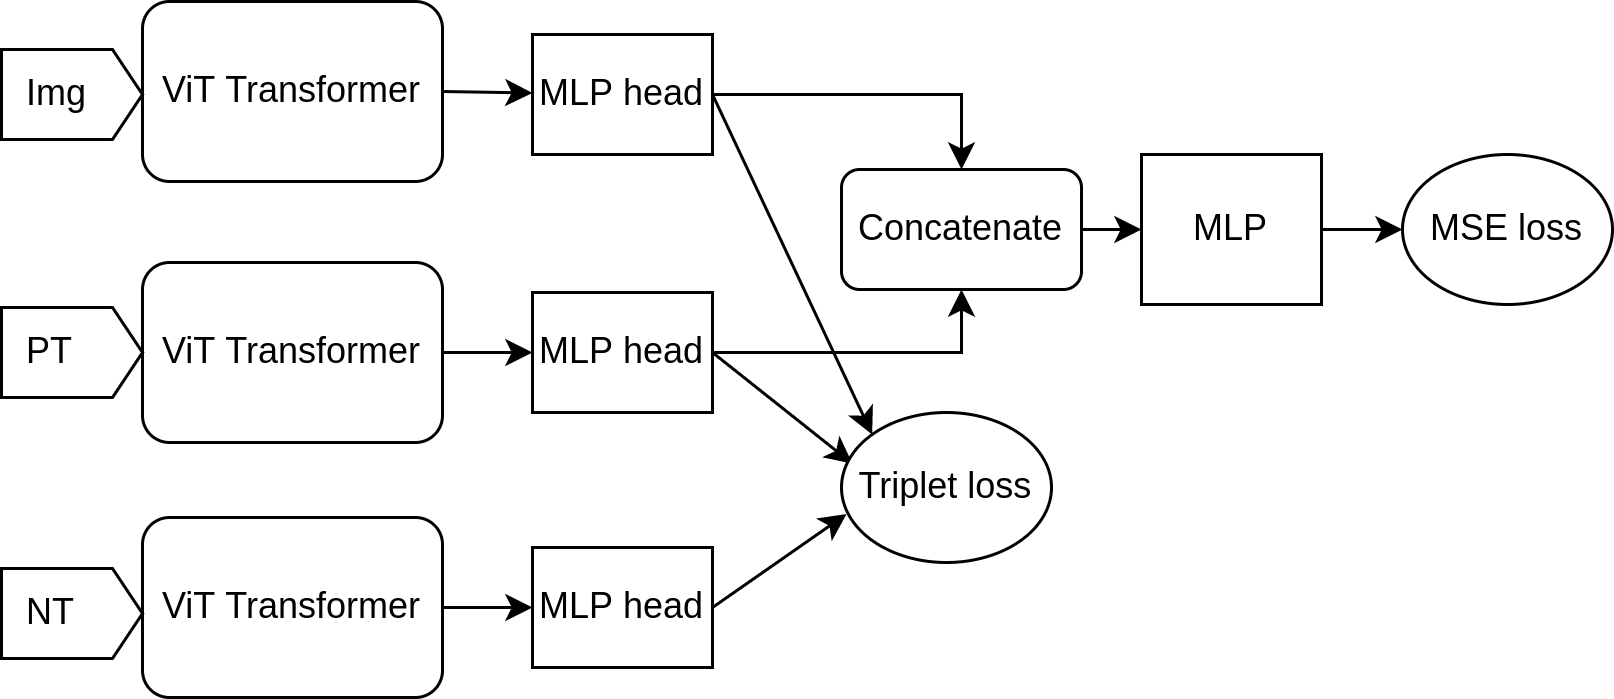
\includegraphics[width=14cm]{second_approach_diagram}
    \caption{The diagram of the second model during training, three siamese transformers for the triplet loss.}
    \label{fig:second_approach_diagram}
\end{figure}

The second model that has been proposed is very similar to the first. The Vit transformer and MLP heads have the same structure, but one extra of them has been added.

The first model takes as input the inspected image and a random template. As shown in figure \ref{fig:second_approach_diagram}, this second model accepts the inspected image, a positive template, and a negative template. This modification was required because this model employs triplet loss rather than cosine embedding loss.

The triplet loss computes image similarity as well, but it requires three inputs instead of a label indicating whether the inputs are similar or not: the input image $a$, a similar template $p$ and a dissimilar template $n$. The triplet loss function is described in \cite{triplet_loss_paper} which is calculated with the formula:
\begin{align*}
    L\left(a,p,n\right) = \max(d(a, p) - d(a, n) + margin, 0)
\end{align*}
where d is a distance swap further described in the paper\cite{triplet_loss_paper}.

We repeat the process for bounding box prediction, but only on the inspected image and positive template, where we concatenate the feature vectors and feed them into the MLP, which generates four coordinate values. We also employ the MSE loss on this part of the network.

Because this model solved the problem of attempting to predict a negative template in the inspected image, these superfluous gradients were removed. At the same time, the model learns image similarity and will be able to predict whether or not a template exists in the inspected image.

This model structure differs for the evaluation phase because our task is to determine whether there is a template in the image and, if so, where it is, which requires only two inputs, not three.

\begin{figure}[htp]
    \centering
    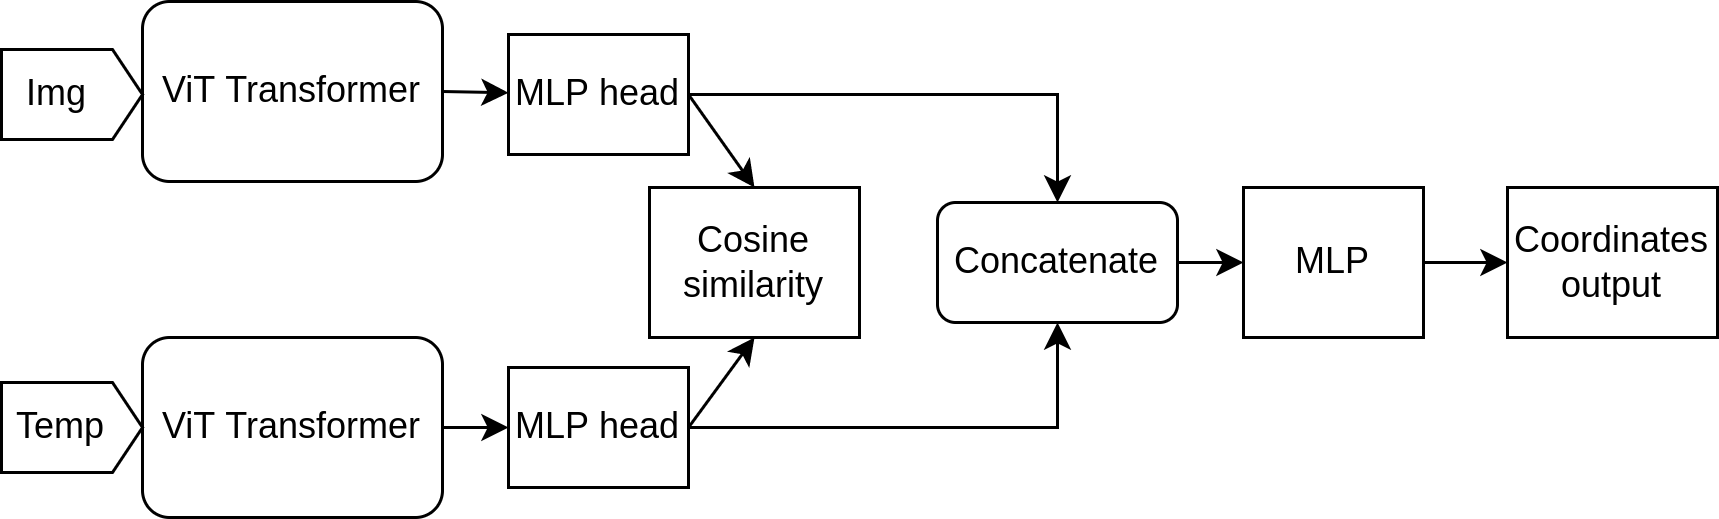
\includegraphics[width=14cm]{second_approach_diagram_eval}
    \caption{The diagram of the second model during evaluation.}
    \label{fig:second_approach_diagram_eval}
\end{figure}

The fact that we first predict whether there is a template in the inspected image using cosine similarity, and then predict the bounding box if there is, fits perfectly with how we trained our model, the triplet loss was trained without interference and learned the similarity notion and the MSE loss was only applied on positive templates, which is exactly what we needed for evaluation.

\chapter{Experiments and results}

\section{Datasets}

In this thesis I have used two datasets, both from the traffic computer vision field.

\textbf{The first dataset} I used for the majority of my experiments is \citefield{carplate_dataset_paper}{title}\cite{carplate_dataset_paper} consisting of over 300000 images of cars from a perspective that shows their car plate. The main task here is to template match the car plate and distinguish between different car plates.

I only used 5000 images to train my model, due to the limited computing resources I had.

\textbf{The second dataset} that I used is the \citefield{traffic_sign_dataset_paper}{title}\cite{traffic_sign_dataset_paper} which contains 100000 images from the traffic containing approximately 30000 traffic sign instances. This dataset includes a set of road sign templates.

\begin{figure}[htp]
    \centering
    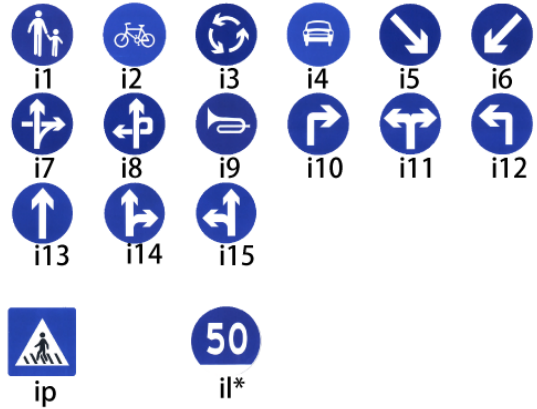
\includegraphics[width=6cm]{traffic_sign_templates}
    \caption{The templates selected from the dataset. Figure from \cite{traffic_sign_dataset_paper}.}
    \label{fig:traffic_sign_templates}
\end{figure}

I chose only a subset of images that contain only the templates depicted in figure \ref{fig:traffic_sign_templates}, so the total number of templates I used from this dataset is 18. I also only chose images with a single instance of a template because the vision transformer model I used can only predict a single instance of an object. I also chose only 5000 images from this dataset to train on.


\section{Implementation details}

The ViT model is obtained from the HuggingFace model list, the exact model I used is Google's vit-base-patch16-224 with input size $224\times224$ pixels divided into $16\times16$ patches. This model is a base model, which means it has 12 stacked encoder layers.

The images from the datasets are preprocessed in two ways:
\begin{enumerate}
    \item manually resized the images to match the input of the transformer
    \item used Google's preprocessing function they used during pre-training. It resizes the image and applies normalization on the image.
\end{enumerate}
Because the dataset images come in pairs of image and template label, we had to choose between a positive template and a negative template with a 50\% probability (so the dataset is balanced) before passing it to the first model.

For both models that were implemented, I frozen a number of transformer encoder layers. I frozen 8 layers for the first model and 10 layers for the second. One of the primary causes of the frozen layers is the limited computational resources used in the experiments. However, freezing transformer layers prevents overfitting the model, and given the small amount of data used, the model is better trained with frozen layers.

Because the two losses I used for training were initially unbalanced, the model was unable to learn at all, so I had to introduce a constant $C$ to bring the two losses closer to each other. I set this variable $C=100$ for the first model and $C=50$ for the second, and divided the similarity loss value by this variable. The total loss formula is as follows:
\begin{align*}
    \text{loss} = \text{MSE\_loss} + \frac{\text{similarity\_loss}}{C}
\end{align*}

% The model model outputs for the cosine similarity a value in the interval , therefore to obtain something comparable to a binary label, and considering that the margin value of the loss is 0.5 we round the prediction:

The model model outputs a value in the interval $\left[-1,1\right]$ for cosine similarity, so to obtain something comparable to a binary label, and given that the loss margin is 0.5, we round the prediction as follows:
\begin{align*}
    \text{prediction} =
        \begin{cases}
        1,  & \text{if } \text{cosine\_similarity} > 0.5 \\
        -1, & \text{if } \text{cosine\_similarity} \leq 0.5
        \end{cases}
\end{align*}

Given the predictions and labels, I used a simple division between the number of positive predictions and the total number of predictions to calculate the accuracy of the similarity between the template and the image.
\begin{align*}
    \text{accuracy}\left(\text{predictions}, \text{labels}\right) = \frac{\text{PP}}{\text{TP}}
\end{align*}

In the case of the bounding box, the model predicts values scaled down to the interval $\left[0,1\right]$, therefore we simply multiply these coordinates by the image size to scale them back.

For the bounding box accuracy, I calculated the intersection over union of the predicted box and the label box, and three accuracies based on how many of the predictions had 50\%, 75\%, respectively, 90\% area intersection with the label.

\section{Experiments}

The experiments were made on a GPU machine with 4 GB of VRAM and 16 GB of RAM.

The results presented in this section are only the best I could get using various parameter configurations. I also replaced the ViT model with the DINO model \cite{dino_paper}, but the results were very similar, so I've only shown the results from the original model.

% On the first dataset I've tried both proposed models. Both models were trained and validated on a total of 5000 images from the car plate dataset, for 20 epochs. I used the AdamW optimizer with a learning rate of  for the consine embedding loss model and  for the triplet loss model.

\subsection{Car plate dataset}

I tried both proposed models on the first dataset. Both models were trained and validated on 5000 images from the car plate dataset, for 20 epochs. For both models, I used the AdamW optimizer, with a learning rate of $2\cdot10^{-4}$ for the consine embedding loss and $1\cdot10^{-4}$ for the triplet loss model.
\begin{figure}[htp]
    \centering
    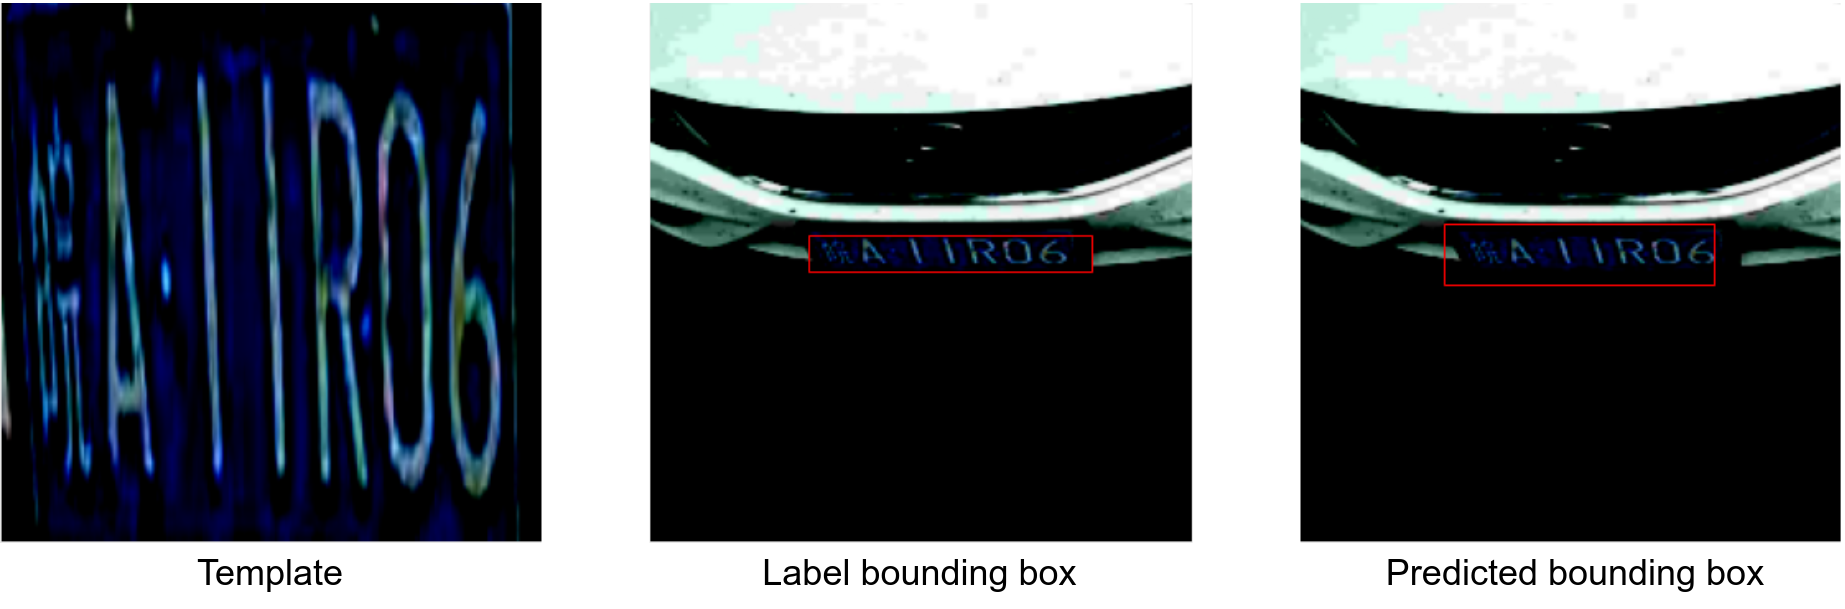
\includegraphics[width=14cm]{prediction_image_cosine_model}
    \caption{Example of a prediction from the first model.}
    \label{fig:prediction_image_cosine_model}
\end{figure}

% \begin{table}[ht]
%     \begin{tabular}{|l|c|c|c|c|}
%     \hline
%               & \multicolumn{1}{l|}{Similarity accuracy} & \multicolumn{1}{l|}{IOU 50\%} & \multicolumn{1}{l|}{IOU 75\%} & \multicolumn{1}{l|}{IOU 90\%} \\ \hline
%     Train      & 86.68\%                                  & 100\%                         & 100\%                         & 75.8\%                        \\ \hline
%     Validation & 85.6\%                                   & 100\%                         & 99\%                          & 74.8\%                        \\ \hline
%     \end{tabular}
%     \centering
%     \caption{The cosine embedding loss model results.}
%     \label{table:first_model_accuracies}
% \end{table}

\begin{table}[ht]
    \begin{tabular}{lcccc}
    \hline
                & Similarity accuracy    & IOU 50\%  & IOU 75\%  & IOU 90\%  \\ \hline
    Train       & 86.68\%                & 100\%     & 100\%     & 75.8\%    \\ \hline
    Validation  & 85.6\%                 & 100\%     & 99\%      & 74.8\%    \\ \hline
    \end{tabular}
    \centering
    \caption{The cosine embedding loss model results.}
    \label{table:first_model_accuracies}
\end{table}

The results of the first model are presented in the table \ref{table:first_model_accuracies}.

As can be seen, the first strategy learns to predict whether the template is present in the inspected image with an accuracy of over 85\%. Considering only these correct similarity predictions, the model further predicts the bounding boxes with an accuracy of 75\% for the 90\% IOU accuracy. These results are acceptable in general, but far beyond what a transformer should be able to predict, considering how simple the dataset is.

% \begin{table}[ht]
%     \begin{tabular}{|l|c|c|c|c|}
%     \hline
%               & \multicolumn{1}{l|}{Similarity accuracy} & \multicolumn{1}{l|}{IOU 50\%} & \multicolumn{1}{l|}{IOU 75\%} & \multicolumn{1}{l|}{IOU 90\%} \\ \hline
%     Train      & 98.03\%                                  & 100\%                         & 99.6\%                        & 65.6\%                        \\ \hline
%     Validation & 92\%                                     & 100\%                         & 97.1\%                        & 50.4\%                        \\ \hline
%     \end{tabular}
%     \centering
%     \caption{The triplet loss model results.}
%     \label{table:second_model_accuracies}
% \end{table}

\begin{table}[ht]
    % \begin{tabular}{|l|c|c|c|c|}
    \begin{tabular}{lcccc}
    \hline
                & Similarity accuracy   & IOU 50\%  & IOU 75\%  & IOU 90\%  \\ \hline
    Train       & 98.03\%               & 100\%     & 99.6\%    & 65.6\%    \\ \hline
    Validation  & 92\%                  & 100\%     & 97.1\%    & 50.4\%    \\ \hline
    \end{tabular}
    \centering
    \caption{The triplet loss model results.}
    \label{table:second_model_accuracies}
\end{table}

The second second approach obtained slightly better results in the similarity perspective, that can be observer in table \ref{table:second_model_accuracies}.

This model performs better on the similarity prediction but it does much worse on the 90\% IOU accuracy, obtaining only $50.4\%$, but even so it still has an accuracy of $97.1\%$ on the 75\% IOU accuracy.

As a reference, we compare our results to those obtained by the database authors using their own model as well as other well-known architectures. We present a comparison between these models and our presented model, comparing its similarity, IOU accuracy and the number of images processed per second (FPS). Table \ref{table:results_comparison} illustrates the comparison.

% \begin{table}[ht]
%     \begin{tabular}{|l|c|c|c|}
%     \hline
%                                         & FPS & Similarity accuracy & IOU accuracy    \\ \hline
%     SSD300\cite{ssd300}                 & 40  & 98.3\%              & 99.1\%          \\ \hline
%     YOLO9000\cite{yolo9000}             & 42  & 98.1\%              & 98.8\%          \\ \hline
%     Faster-RCNN\cite{faster_rcnn_paper} & 15  & 97.2\%              & 98.1\%          \\ \hline
%     TE2E\cite{te2e}                     & 3   & 97.8\%              & 98.5\%          \\ \hline
%     RPnet\cite{carplate_dataset_paper}  & 61  & \textbf{98.5\%}     & \textbf{99.3\%} \\ \hline
%     \textbf{Cosine model}               & 35  & 85.6\%              & 99\%            \\ \hline
%     \textbf{Triplet model}              & 25  & 92\%                & 97.1\%          \\ \hline
%     \end{tabular}
%     \centering
%     \caption{Comparison with other models results, taken from \cite{carplate_dataset_paper}}
%     \label{table:results_comparison}
% \end{table}
\begin{table}[ht]
    % \begin{tabular}{|lccc|}
    \begin{tabular}{lccc}
    \hline
                                        & FPS           & Similarity accuracy & IOU accuracy    \\ \hline
    SSD300\cite{ssd300}                 & 40            & 98.3\%              & 99.1\%          \\ \hline
    YOLO9000\cite{yolo9000}             & 42            & 98.1\%              & 98.8\%          \\ \hline
    Faster-RCNN\cite{faster_rcnn_paper} & 15            & 97.2\%              & 98.1\%          \\ \hline
    TE2E\cite{te2e}                     & 3             & 97.8\%              & 98.5\%          \\ \hline
    RPnet\cite{carplate_dataset_paper}  & \textbf{61}   & \textbf{98.5\%}     & \textbf{99.3\%} \\ \hline
    \textbf{Cosine model}               & 35            & 85.6\%              & 99\%            \\ \hline
    \textbf{Triplet model}              & 25            & 92\%                & 97.1\%          \\ \hline
    \end{tabular}
    \centering
    \caption{Comparison with other models results which are taken from \cite{carplate_dataset_paper}.}
    \label{table:results_comparison}
\end{table}

The above results are only used as a reference because they were trained on 100.000 data samples and a different GPU was used; however, because our environments are generally similar, it is a good comparison.

The validation similarity accuracy of the models can be seen in figure \ref{fig:similarity_accuracy_model_comparison}, and as we can observe the models tend to finish learning by the time they reach epoch 20.

% The IOU accuracies plots can be seen in figure \ref{fig:iou_accuracies_model_comparison}, which for the cosine embedding loss seems to be pretty stable but it's very unstable for the triplet loss model. I've attempted to train the triplet loss model for more than 20 epochs, but training for more only overfits the model.

The IOU accuracies plots can be seen in figure \ref{fig:iou_accuracies_model_comparison}, which appear to be fairly stable for the cosine embedding loss model but very unstable for the triplet loss model. I tried training the triplet loss model for more than 20 epochs with a smaller learning rate, but doing so just overfits the model.

The loss of the models corresponds to the accuracy evolution of the models, as depicted in figure \ref{fig:loss_model_comparison}. The triplet loss model, once again, has a more unstable loss evolution caused by the bounding box regression loss.

\subsection{Traffic sign dataset}

I only used the first proposed model on the traffic sign dataset. This dataset is difficult for the transformer because the input images are $1920\times1080$ pixels, and the traffic signs are also very small as seen in figure \ref{fig:roadsign_dataset_example}, so when resized to 224 pixels, it loses too much pixel information.

\begin{figure}[htp]
    \centering
    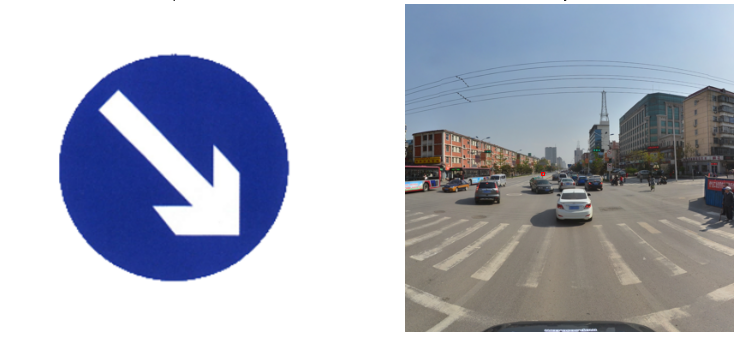
\includegraphics[width=12cm]{roadsign_dataset_example}
    \caption{The template and the labelled inspected image. Sample from second dataset.}
    \label{fig:roadsign_dataset_example}
\end{figure}


On this dataset, the model produces poor results, with an accuracy of less than 10\% on a 90\% IOU accuracy. I've also tried using a different version of the ViT model with $384\times384$ images as input, but the results aren't any better.

\section{Ablation study}

To see how essential the similarity component of the model is, I removed the cosine embedding loss part from the first model we looked at, and instead of using a random template, I only utilized templates that were present in the examined image.

We trained the model with the same procedure as the whole model.

This model only had a 50\% accuracy on the 90\% IOU, indicating that the similarity component of the model is critical, as it not only allows the model to predict whether there is a template in the image, but it also aids in the prediction of the bounding box.

\begin{figure}[!htp]
    \centering
    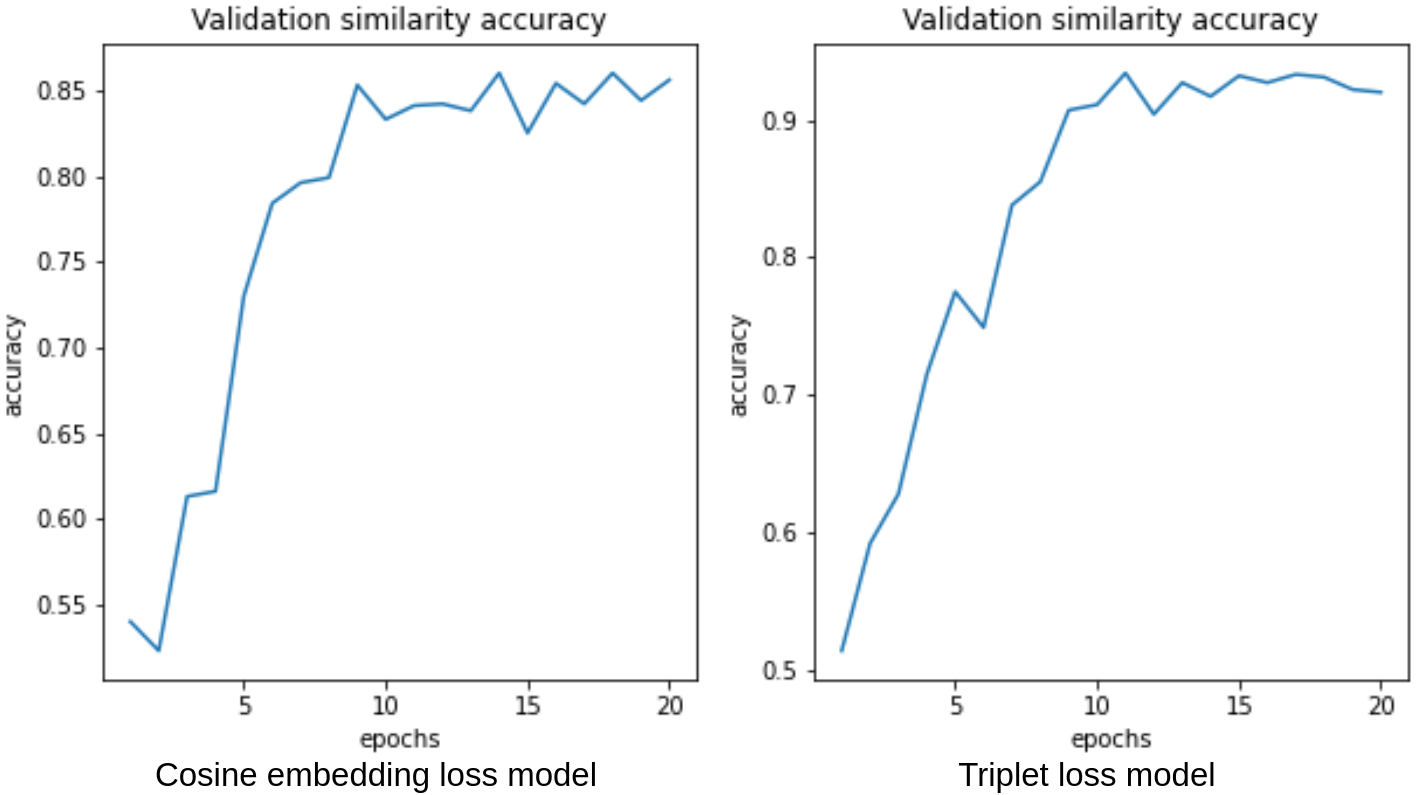
\includegraphics[width=12cm]{similarity_accuracy_model_comparison}
    \caption{The plots of the similarity accuracy of the two models.}
    \label{fig:similarity_accuracy_model_comparison}
\end{figure}

\begin{figure}[!htp]
    \centering
    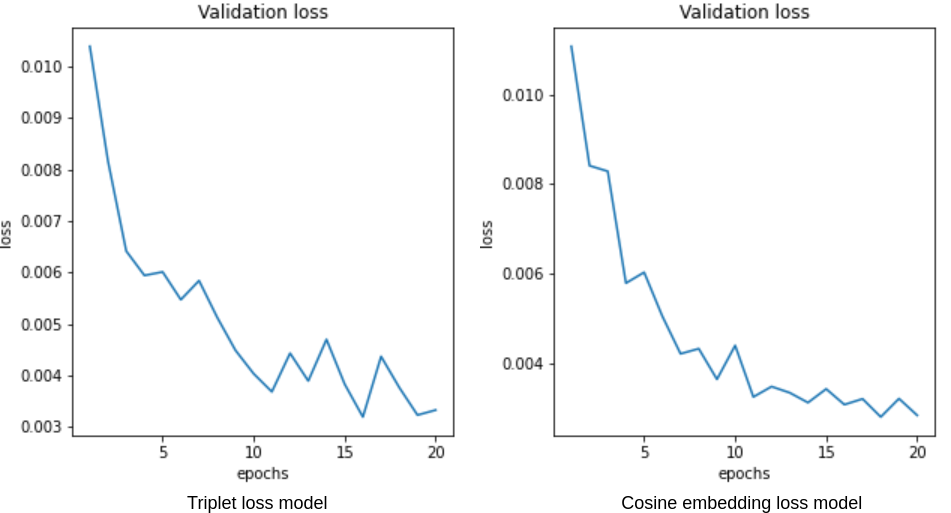
\includegraphics[width=12cm]{loss_model_comparison}
    \caption{The plots of the loss of the two models on the first dataset.}
    \label{fig:loss_model_comparison}
\end{figure}

\begin{figure}[htp]
    \centering
    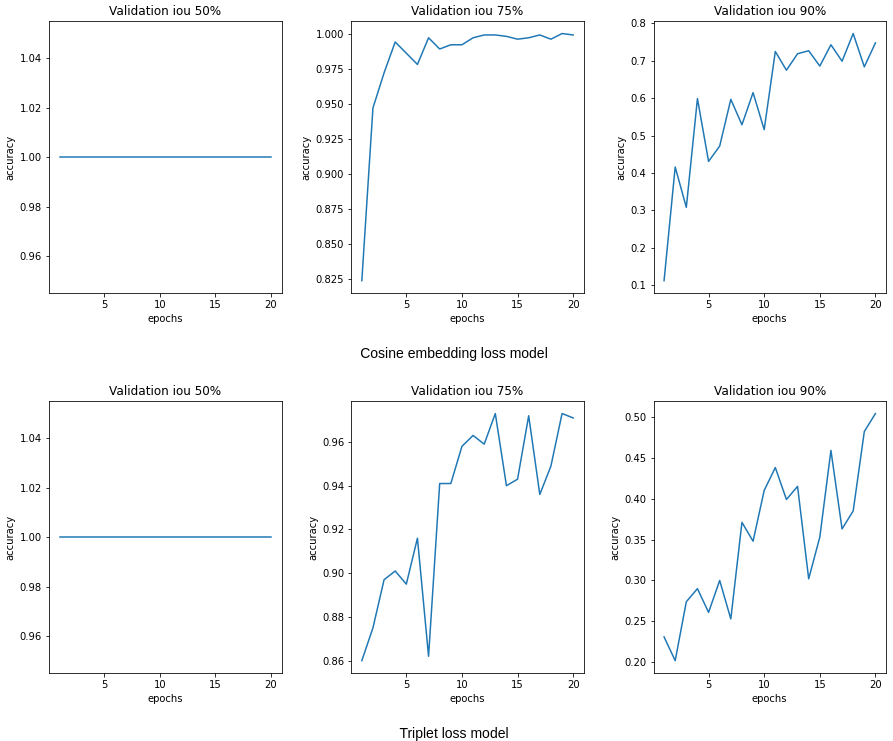
\includegraphics[width=15cm]{iou_accuracies_model_comparison}
    \caption{The plots of the IOU accuracy of the two models on the first dataset.}
    \label{fig:iou_accuracies_model_comparison}
\end{figure}

\chapter{Conclusion and further research}

\section{Conclusion}

The implemented models were capable of learning how to perform object recognition based on a given template. As a result, transformers can be used in template matching using siamese networks.

In the first dataset, we observed the difference between the two approaches presented. The first model produces reasonably good and consistent results, but the second model was designed to not only predict better in the similarity aspect, but also to improve the bounding box accuracy, which I suspected was hampered by the model's attempt to predict negative templates. 

However, as we have seen, it performs better in terms of similarity but loses a lot of accuracy in terms of bounding box prediction.

The model was unable to predict anything for the second dataset, which I suspect is because the ViT model was pre-trained on a classification task with large object representations, so the model does not pay attention to the small objects.

Overall, the experiments were conducted on a very small portion of the dataset and with the majority of the transformer layers frozen. Thus, the main goal was to see if a transformer-based model could learn to template match, which we were able to do.

\section{Further research}

To fully explore the potential of the models, we would need to train the models on the entire dataset and with fewer frozen transformer layers, so this will need to be further experimented with with the corresponding computational resources.

Template matching implies matching all instances from an image, not just one. Although some transformer models that can predict multiple objects and classes have been developed\cite{detr_paper}\cite{yolos_paper}, they still perform worse than the CNN-based state-of-the-art. As a result, the concept of multiple object detection using a transformer should be further investigated.

Considering how BERT\cite{bert_paper} was designed on the input perspective, a similar transformer design but for images might be the most optimal way to perform template matching, although training such a model would be very expensive computationally.

\printbibliography[heading=bibintoc]

\end{document}